% !TEX program = xelatex

\RequirePackage{silence}
\WarningFilter{babel}{Name 'brazil' is deprecated}
\WarningFilter{memoir}{\settocpreprocessor}

\documentclass[
  12pt,
  a4paper,
  oneside,
  chapter=TITLE,
  english,
  brazil
]{abntex2}

\usepackage{fontspec}
\setmainfont{Arial}
\setsansfont{Arial}
\setmonofont{Arial}

\usepackage{microtype}
\usepackage{indentfirst}
\usepackage{calc}
\usepackage{graphicx}

\providecommand{\captionsetup}[1]{\renewcommand{\tablename}{Quadro}}
\addto\captionsbrazil{\renewcommand{\listtablename}{Lista de quadros}}
\renewcommand{\cfttablename}{Quadro }

\usepackage{amsmath,amssymb}
\usepackage{longtable,booktabs,array}
\AddToHook{env/longtable/begin}{\renewcommand{\_}{\textunderscore\allowbreak}}
\newcommand{\real}[1]{#1}
\usepackage{xcolor}

\usepackage[alf]{abntex2cite}
\bibliographystyle{abntex2-alf}

\usepackage{hyperref}
\hypersetup{hidelinks}

\setlength{\parindent}{1.25cm}
\OnehalfSpacing

\instituicao{INSTITUTO FEDERAL DE EDUCAÇÃO, CIÊNCIA E TECNOLOGIA DE SÃO PAULO}
\autor{BRIAN GUSTAVO DE OLIVEIRA BRANDÃO}
\titulo{MEGAGAME: SISTEMA DE MARKETPLACE DE JOGOS}
\local{Campos do Jordão}
\data{2026}
\tipotrabalho{Projeto Integrador}
\orientador{[NOME DO(A) ORIENTADOR(A)]}
\preambulo{Projeto Integrador apresentado ao Instituto Federal de Educação,
Ciência e Tecnologia de São Paulo (IFSP), Campus Campos do Jordão, como
requisito parcial para obtenção do título de Tecnólogo em Análise e
Desenvolvimento de Sistemas.}

\begin{document}
\selectlanguage{brazil}

\pretextual

\hypersetup{pageanchor=false}
\imprimircapa
\hypersetup{pageanchor=true}
\imprimirfolhaderosto

\begin{folhadeaprovacao}
  \begin{center}
    {\ABNTEXchapterfont\large\imprimirautor}

    \vspace*{\fill}\vspace*{\fill}
    \begin{center}
      \ABNTEXchapterfont\bfseries\Large\imprimirtitulo
    \end{center}
    \vspace*{\fill}

    \hspace{.45\textwidth}
    \begin{minipage}{.5\textwidth}
      \imprimirpreambulo
    \end{minipage}%
    \vspace*{\fill}
  \end{center}

  Trabalho aprovado. \imprimirlocal, [DATA DA DEFESA]:

  \assinatura{\textbf{\imprimirorientador} \\ Orientador(a)}
  \assinatura{\textbf{[NOME DO(A) AVALIADOR(A) 1]} \\ Avaliador(a)}
  \assinatura{\textbf{[NOME DO(A) AVALIADOR(A) 2]} \\ Avaliador(a)}
\end{folhadeaprovacao}

\begin{resumo}
Este documento apresenta o desenvolvimento de um \emph{marketplace} C2C
chamado MegaGame. É voltado para a área de jogos, principalmente os
eletrônicos, mas também permitindo a comercialização de diversos itens
associados. Tal mercado vem crescendo de forma dramática com o passar
dos anos, tanto em retorno financeiro quanto em número de interessados,
algo que populariza serviços relacionados ao setor e lhes torna cada vez
mais comercialmente viáveis. Com esse contexto em mente, o projeto busca
justamente construir um sistema que seja funcional e atrativo para os
clientes, sejam eles vendedores, compradores ou ambos simultaneamente.

\textbf{Palavras-chave:} \emph{marketplace}; jogos; gerenciamento; clientes.
\end{resumo}

\begin{resumo}[Abstract]
\begin{otherlanguage*}{english}
This document presents the development of a C2C marketplace called
MegaGame. Its focus is on the gaming sector, especially electronic
games, but also allowing for the commercialization of several related
items. The market has been growing dramatically over the years, not only
in financial return but also in number of prospective clients, which
means related services have become increasingly more popular and
commercially viable. With that context in mind, the project aims to
build a system that is functional and attractive to clients, whether
they're buyers, sellers or both simultaneously.

\textbf{Keywords:} marketplace; games; management; clients.
\end{otherlanguage*}
\end{resumo}

\begin{siglas}
  \item[C2C] \emph{Customer-to-customer}
  \item[SGBD] Sistema de gerenciamento de banco de dados
  \item[SSR] \emph{Server-side rendering}
\end{siglas}

\pdfbookmark[0]{\contentsname}{toc}
\tableofcontents*
\listoffigures*
\listoftables*

\textual

\chapter{Introdução}

A indústria de jogos eletrônicos atualmente forma um dos maiores
mercados da área de entretenimento, movimentando centenas de bilhões de
dólares ao todo. Segundo pesquisas como as da \citeonline{newzooTopCountries}, Brasil costuma
estar entre os dez países que mais contribuem para tal situação,
possuindo uma forte comunidade \emph{gamer}.

Sendo assim, este projeto tem como objetivo apresentar um
\emph{marketplace} C2C chamado MegaGame, voltado para essa audiência.
Além da oportunidade comercial, o desenvolvimento do site também foi
motivado pela observação do autor de que seria útil existir um local
centralizado para o comércio de itens relacionados ao tema, tendo em
vista a grande dispersão através de diversas plataformas (OLX, Mercado
Livre, Shopee, dentre outras) em decorrência da falta de um serviço
dedicado ao segmento.

Para o desenvolvimento do MegaGame, foram utilizados a linguagem Python
(com o \emph{framework} Django) e o SGBD PostgreSQL (através da
plataforma Supabase).

\section{Objetivos}

O objetivo da plataforma criada neste trabalho é fornecer um serviço
eficiente, intuitivo, estável e responsivo, utilizando tecnologias
difundidas no ramo da tecnologia para viabilizar esses requisitos. Já o
objetivo deste documento em específico é descrever toda a criação do
MegaGame, detalhando o processo de desenvolvimento e fornecendo
informações sobre suas funcionalidades e casos de uso.

\section{Justificativa}

Conforme citado anteriormente, a justificativa deste trabalho se dá pela
observação do autor de que há uma lacuna (ao menos no cenário
brasileiro) na indústria de \emph{games} que pode ser preenchida por uma
plataforma com as características do MegaGame, além da crescente
viabilidade comercial do setor.

Logo, o sistema se torna ideal tanto para os clientes quanto para seu(s)
gestor(es), demonstrando assim sua relevância para todos os
\emph{stakeholders} envolvidos, conforme ressaltam os conteúdos
referentes à gestão de projetos abordados durante o curso.

\section{Aspectos metodológicos}

As ferramentas utilizadas durante a criação do projeto foram a linguagem
de programação Python no \emph{back end}, através do \emph{framework}
Django e utilizando a prática de SSR; a linguagem de programação
JavaScript no \emph{front end}, aliada às linguagens de \emph{markdown}
e \emph{style sheets} HTML e CSS (respectivamente); e além disso, o SGBD
PostgreSQL, através da plataforma online Supabase para hospedagem na
nuvem.

Já a ferramenta utilizada para criação dos diagramas da linguagem de
modelagem UML exibidos no documento foi o draw.io, mais especificamente
sua versão \emph{web} (também chamada de diagrams.net).

\section{Aporte teórico}

Para os estudos teóricos acerca do tema abordado, foram consultados
alguns dos livros mais populares e acessíveis sobre tópicos como o UML,
a engenharia de \emph{software} e o gerenciamento de bancos de dados,
além de fontes virtuais que comprovem alguns dos conceitos que embasam o
projeto como um todo.

Mais especificamente, os escritos de autores como Coronel, Pressman e
etc. foram as responsáveis por ajudar a definir os princípios guiadores
do trabalho, graças aos métodos, práticas e paradigmas estabelecidos e
discutidos por tais obras.

\chapter{Fundamentação teórica}

Nesta seção, serão apresentadas em maiores detalhes as tecnologias e
teorias empregadas durante a construção do projeto.

\section{Engenharia de software}

O conceito de engenharia de \emph{software} é utilizado para se referir
a uma área da computação voltada para a aplicação de certos princípios e
ferramentas, com o intuito de esquematizar, desenvolver e gerenciar
sistemas. Seu propósito é garantir que todos os requisitos determinados
no início de um projeto sejam cumpridos de forma eficaz, mas também de
forma eficiente quando possível; isto é, assegurando que tudo esteja
dentro do prazo estabelecido, respeitando os limites orçamentários e se
encaixando em padrões de qualidade do mercado (como as normas ISO, por
exemplo).

Atualmente, no contexto acadêmico, são duas as principais referências
neste setor -- as obras de Pressman e Maxim, junto das obras de
Sommerville. \citeonline[p. 59]{pressman2021engenharia} dizem, acerca do tema:

\begin{quote}
O Instituto de Engenheiros Eletricistas e Eletrônicos (IEEE) elaborou a
seguinte definição para engenharia de \emph{software}: {[}...{]} a
aplicação de uma abordagem sistemática, disciplinada e quantificável no
desenvolvimento, na operação e na manutenção de \emph{software}; isto é,
a aplicação de engenharia ao \emph{software}.
\end{quote}

Já \citeonline[p. 22]{sommerville2011engenharia} afirma:

\begin{quote}
A engenharia de \emph{software} tem por objetivo apoiar o
desenvolvimento profissional de \emph{software}, mais do que a
programação individual. Ela inclui técnicas que apoiam especificação,
projeto e evolução de programas, que normalmente não são relevantes para
o desenvolvimento de \emph{software} pessoal.
\end{quote}

As etapas da engenharia de \emph{software} são organizadas em processos,
para os quais são levantados os requisitos correspondentes. Assim, os
melhores métodos possíveis podem ser empregados para cumpri-los.

\subsection{Análise de requisitos}

Existem três tipos diferentes de requisito, sendo dois deles os
principais (mais precisamente, os funcionais e os não-funcionais).
Primeiramente, os requisitos funcionais descrevem as funcionalidades
exatas que um sistema deve possuir. Por exemplo, um site que trabalhe
com perfis de usuário deve permitir que seus clientes cadastrem contas
para si e depois efetuem o \emph{login} nelas.

Já os requisitos não-funcionais referem-se aos atributos de qualidade
que o sistema deve alcançar. Por instância, suportar X usuários
simultâneos, carregar todo o conteúdo em até Y segundos, garantir
conformidade com leis de proteção de dados de determinado território,
dentre outros casos.

E por fim, existem também os requisitos de domínio. Tecnicamente, eles
irão cair dentro de uma das categorias anteriores, mas vale a pena
ressaltá-los a parte pois correspondem às regras de negócio de um
determinado setor; isto é, são formados a partir da análise daquela área
em específico, para garantir que suas particularidades estejam sendo
observadas e tratadas.

Para obter todos os requisitos, é realizada uma ação conhecida como
levantamento, que pode englobar várias táticas. Análise de mercado,
entrevistas com peritos, discussões de ideias com o cliente e/ou outros
desenvolvedores (processo também conhecido como \emph{brainstorming}) e
demais práticas são passíveis de serem utilizadas durante essa etapa do
planejamento.

\subsection{Modelagem}

A partir do momento em que os requisitos foram todos levantados e já
existe uma ideia do rumo que o projeto deve tomar, é uma boa prática
fazer a modelagem do \emph{software}, através de ferramentas como o UML
(cujo uso será mais detalhado posteriormente, por se tratar de uma
linguagem utilizada durante a construção deste trabalho em específico).

Modelagem, neste cenário, significa representar o sistema sendo
desenvolvido através de recursos visuais, facilitando sua compreensão,
análise e posterior implementação. É especialmente útil para trabalhos
em equipe ou que envolvem \emph{stakeholders} externos, mas também pode
se mostrar de suma importância mesmo em criações individuais.

Ela pode abranger diversas áreas. No ecossistema da UML, por exemplo,
existem diagramas de casos de uso, diagramas de classe (que representam
a estrutura do sistema, através do conceito da programação orientada a
objetos), diagramas de sequência (para detalhar as atividades que o
sistema realiza), dentre outros.

\section{Linguagens e ferramentas utilizadas}

\subsection{UML}

UML significa Unified Modeling Language (``linguagem unificada de
modelagem'', em inglês), que é o nome de uma linguagem de modelagem
desenvolvida na década de 1990 por Grady Booch, James Rumbaugh e Ivar
Jacobson, a partir da unificação de suas três linguagens desenvolvidas
de forma independente em um ``pacote'' coeso.

\begin{figure}[htbp]
  \centering
  
\includegraphics[width=0.8\textwidth]{images/image1.png}
  \caption{Logo da UML}
  \label{fig:uml-logo}
  \legend{Fonte: \citeonline{wikipediaUmlLogo}.}
\end{figure}

Desde 1997, a UML é gerida e padronizada pelo Object Management Group
(ou OMG). Possui diversos usuários no meio de desenvolvimento de
\emph{software}, inclusive Gilleanes Guedes, cujas obras servem como um
guia para sua utilização ideal. \citeonline[p. 24]{guedes2018uml} afirma:

\begin{quote}
Um modelo de software captura uma visão de um sistema físico; é uma
abstração do sistema com um certo propósito, como descrever aspectos
estruturais ou comportamentais do \emph{software}. Esse propósito
determina o que deve ser incluído no modelo e o que é considerado
irrelevante. Assim, um modelo descreve completamente aqueles aspectos do
sistema físico relevantes ao propósito do modelo, no nível apropriado de
detalhe.
\end{quote}

Os diagramas da UML são divididos em dois tipos: os estruturais e os
comportamentais. Os primeiros focam na organização estática do sistema
(como os diagramas de classes, objetos, componentes, implantação...) e
os últimos focam na dinâmica e interações do sistema (como os diagramas
de casos de uso, sequência, estados...)

\subsection{Django}

O Django é um \emph{framework} para a linguagem Python, desenvolvido em
2005 por Adrian Holovaty e Simon Willison, sendo mantido desde então
pela Django Software Foundation. O Python, por sua vez, fora
desenvolvido em 1991 pelo neerlandês Guido van Rossum para suceder uma
linguagem anterior conhecida como ABC, e é uma das linguagens de
programação mais populares e acessíveis do mundo.
\begin{figure}[htbp]
  \centering
  
\includegraphics[width=0.6\textwidth]{images/image2.png}
  \caption{Logo do Django}
  \label{fig:django-logo}
  \legend{Fonte: \citeonline{wikipediaDjango}.}
\end{figure}

\begin{figure}[htbp]
  \centering
  
\includegraphics[width=0.25\textwidth]{images/image3.png}
  \caption{Logo do Python}
  \label{fig:python-logo}
  \legend{Fonte: \citeonline{wikipediaPythonLogo}.}
\end{figure}


Em comparação com outros \emph{frameworks} para Python, como o Flask, o
Django se destaca por ser voltado ao desenvolvimento \emph{web}. É
utilizado por diversas empresas, incluindo o próprio IFSP, em sua
plataforma virtual SUAP. Trabalha com o conceito de componentes (similar
a alguns outros \emph{frameworks web} populares, como Angular, este em
especíico sendo visto no decorrer do curso), permitindo alta
modularização, e providencia uma interface administrativa embutida para
facilitar a gestão.

\begin{figure}[htbp]
  \centering
  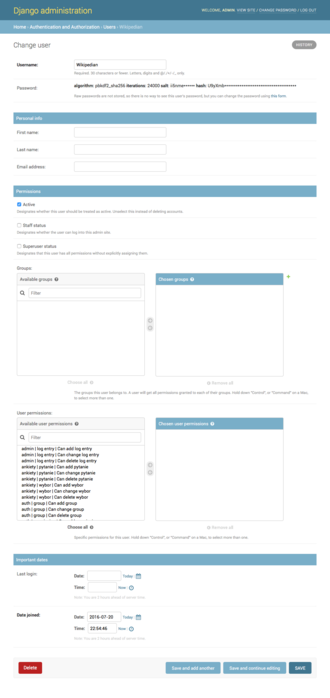
\includegraphics[width=0.55\textwidth]{images/image4.png}
  \caption{Demonstração do painel administrativo do Django}
  \label{fig:django-admin}
  \legend{Fonte: \citeonline{wikipediaDjango}.}
\end{figure}

Através da prática do SSR, é possível utilizá-lo para exibir o site sem
necessidade de \emph{frameworks} adicionais de \emph{front end}. Sendo
assim, se tratando da questão \emph{web}, a combinação usual de
HTML/CSS/JavaScript já foi suficiente pra atingir todas as metas
almejadas.

\subsection{Supabase}

O Supabase é uma plataforma que permite o armazenamento de um banco de
dados na nuvem. Trabalha especificamente com PostgreSQL, mas é possível
fazer a conversão automática do código incluso no repositório do projeto
em trechos correspondentes de SQL que criem as tabelas e campos
necessários no banco, através do processo de \emph{migration}.

Foi criada em 2020 na Singapura por Paul Copplestone e Ant Wilson, como
uma alternativa \emph{open-source} ao Firebase, serviço com uma proposta
similar que é de posse do Google.

\begin{figure}[htbp]
  \centering
  
\includegraphics[width=0.85\textwidth,alt={Logo do Supabase}]{images/image5.jpeg}
  \caption{Logo do Supabase}
  \label{fig:supabase-logo}
  \legend{Fonte: \citeonline{supabaseLogo}.}
\end{figure}

Vale notar que, em testes locais, o SQLite foi utilizado por sua
performance, visto que em tais circunstâncias não era necessário
armazenar o conteúdo gerado a longo prazo.

\section{Desenvolvimento do projeto}

O projeto começou com a ideia inicial, que surgiu a partir dos gostos
pessoais do autor deste trabalho, com o auxílio das sugestões do
orientador da disciplina. A partir dela, foi feita uma pesquisa de
mercado para determinar as regras de negócio do setor, além da confecção
de \emph{wireframes} pras principais páginas do site, de modo a definir
o design geral.
\begin{figure}[htbp]
  \centering
  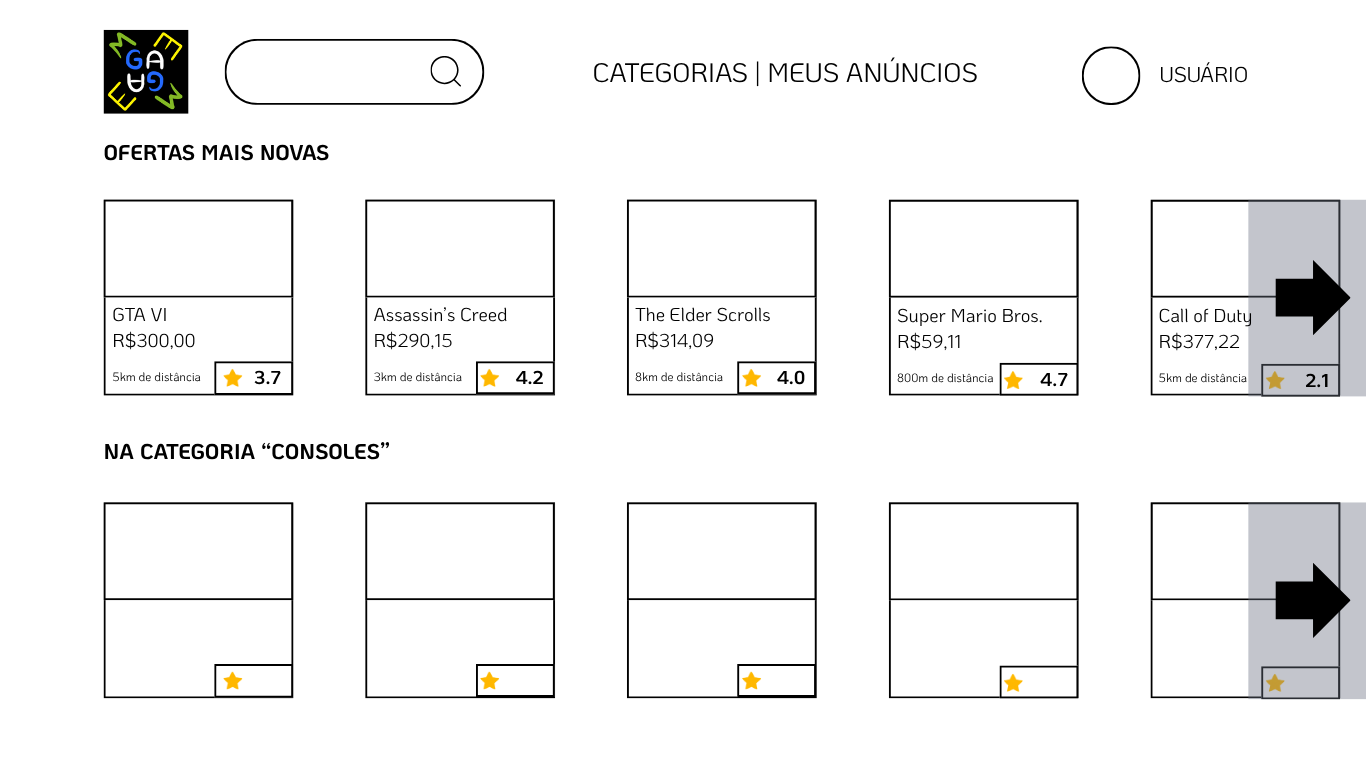
\includegraphics[width=0.9\textwidth]{images/image6.png}
  \caption{\emph{Wireframe} da página inicial do MegaGame}
  \label{fig:wireframe-home}
  \legend{Fonte: Autor (2026).}
\end{figure}


Daí veio o código, sendo que todos os aspectos (\emph{front},
\emph{back} e banco de dados) foram trabalhados simultaneamente. Também
foram feitos testes para tratar exceções e garantir que as
funcionalidades estivessem alinhadas com o escopo do projeto e
protegidas contra brechas de segurança.

Como último passo, veio a formalização da documentação e da modelagem,
conforme demonstrado ao decorrer deste texto.

\chapter{Projeto proposto}

Nesta seção, serão apresentados os detalhes por trás do funcionamento do
MegaGame, além de seus modelos, instruções de uso e \emph{proof of
concept} (prova de conceito) visual.

\section{Considerações iniciais}

Reiterando o que foi supracitado em seções anteriores, o sistema é feito
em Django (com uso de SSR), consequentemente utilizando arquitetura
baseada em componentes, trabalhando assim os conceitos da programação
modular. Para o \emph{front}, foi utilizado HTML/CSS/JavaScript conforme
o padrão do desenvolvimento \emph{web}. E pro banco de dados, foi
empregado o PostgreSQL através da plataforma Supabase para garantir
armazenamento em nuvem.

\section{Requisitos}

Os requisitos funcionais do projeto foram:

{\captionsetup{name=Quadro}
\begin{longtable}[]{@{}
  >{\centering\arraybackslash}p{(\linewidth - 4\tabcolsep) * \real{0.1250}}
  >{\centering\arraybackslash}p{(\linewidth - 4\tabcolsep) * \real{0.6875}}
  >{\centering\arraybackslash}p{(\linewidth - 4\tabcolsep) * \real{0.1875}}@{}}
\caption{Requisitos funcionais}\label{qua:requisitos-funcionais}\\
\toprule\noalign{}
\begin{minipage}[b]{\linewidth}\centering
Código
\end{minipage} & \begin{minipage}[b]{\linewidth}\centering
Requisito
\end{minipage} & \begin{minipage}[b]{\linewidth}\centering
Prioridade
\end{minipage} \\
\midrule\noalign{}
\endfirsthead
\toprule\noalign{}
\begin{minipage}[b]{\linewidth}\centering
Código
\end{minipage} & \begin{minipage}[b]{\linewidth}\centering
Requisito
\end{minipage} & \begin{minipage}[b]{\linewidth}\centering
Prioridade
\end{minipage} \\
\midrule\noalign{}
\endhead
\bottomrule\noalign{}
\endlastfoot
\textbf{RF1} & O sistema deve permitir que o usuário efetue
\emph{login}. & Alta \\
\textbf{RF2} & O sistema deve permitir que novos usuários se cadastrem.
& Alta \\
\textbf{RF3} & O sistema deve permitir a alteração

dos dados de perfil após criação

da conta de usuário. & Alta \\
\textbf{RF4} & O sistema deve manter um histórico completo

de todas as ações realizadas, seja pelo(s)

gestor(es) ou pelos clientes. & Alta \\
\textbf{RF5} & O sistema deve possuir \emph{dashboards}, tanto para o(s)
gestor(es) quanto para os clientes, para que eles possam fazer o
rastreio da parte financeira. & Alta \\
\textbf{RF6} & O sistema deve permitir que o usuário busque

anúncios específicos através de

uma barra de pesquisa. & Média \\
\textbf{RF7} & O sistema deve permitir a compra

e venda de produtos através

de anúncios. & Alta \\
\textbf{RF8} & O sistema deve permitir a edição e

exclusão de anúncios depois que

eles forem ao ar. & Alta \\
\textbf{RF9} & O sistema deve permitir a categorização de produtos. &
Média \\
\textbf{RF10} & O sistema deve permitir a criação de variações para um
produto, cada qual com suas informações específicas (nome, preço,
estoque...) & Média \\
\textbf{RF11} & O sistema deve estar de acordo com as práticas

de responsividade e acessibilidade

vigentes no mercado. & Baixa \\
\textbf{RF12} & O sistema deve permitir que um usuário rastreie todo o
fluxo de envio do produto que comprou

antes de tê-lo em mãos. & Alta \\
\textbf{RF13} & O sistema deve permitir que um usuário tenha o direito
de cancelar seu pedido em determinados momentos, incluindo em um certo
espaço de tempo após a entrega. & Alta \\
\textbf{RF14} & O sistema deve permitir que seus usuários façam
avaliações, tanto dos vendedores dos quais

compraram quanto dos produtos que obtiveram. & Baixa \\
\textbf{RF15} & O sistema deve permitir que seus usuários naveguem pelas
diferentes categorias cadastradas para ver todos os anúncios
pertencentes a determinada categoria. & Baixa \\
\textbf{RF16} & O sistema deve permitir que o gestor

altere a taxa de comissão recebida

sobre as vendas. & Alta \\
\textbf{RF17} & O sistema deve permitir que o comprador possa colocar
produtos em um carrinho, para então finalizar o pedido quando estiver
satisfeito com suas escolhas. & Alta \\
\textbf{RF18} & O sistema deve permitir que uma criação de

anúncio interrompida possa ser

retomada posteriormente. & Média \\
\end{longtable}
\legend{Fonte: Autor (2026).}
}

Já os não-funcionais foram:

{\captionsetup{name=Quadro}
\begin{longtable}[]{@{}
  >{\centering\arraybackslash}p{(\linewidth - 4\tabcolsep) * \real{0.1250}}
  >{\centering\arraybackslash}p{(\linewidth - 4\tabcolsep) * \real{0.6875}}
  >{\centering\arraybackslash}p{(\linewidth - 4\tabcolsep) * \real{0.1875}}@{}}
\caption{Requisitos não funcionais}\label{qua:requisitos-nao-funcionais}\\
\toprule\noalign{}
\begin{minipage}[b]{\linewidth}\centering
Código
\end{minipage} & \begin{minipage}[b]{\linewidth}\centering
Requisito
\end{minipage} & \begin{minipage}[b]{\linewidth}\centering
Prioridade
\end{minipage} \\
\midrule\noalign{}
\endfirsthead
\toprule\noalign{}
\begin{minipage}[b]{\linewidth}\centering
Código
\end{minipage} & \begin{minipage}[b]{\linewidth}\centering
Requisito
\end{minipage} & \begin{minipage}[b]{\linewidth}\centering
Prioridade
\end{minipage} \\
\midrule\noalign{}
\endhead
\bottomrule\noalign{}
\endlastfoot
\textbf{RNF1} & O sistema deve carregar todo o conteúdo

de uma determinada página em até 5 segundos. & Média \\
\textbf{RNF2} & O sistema deve suportar até 1000 usuários

simultâneos sem que haja

perda de desempenho. & Alta \\
\textbf{RNF3} & O sistema deve ser compatível com Windows 10 ou
superior. & Alta \\
\textbf{RNF4} & O sistema deve garantir disponibilidade

mínima de 99\% ao longo

de um ano. & Alta \\
\textbf{RNF5} & O sistema deve estar de acordo

com a LGPD (Lei Geral de

Proteção de Dados). & Alta \\
\textbf{RNF6} & O sistema deve ser projetado para facilitar manutenção e
eventuais atualizações, fazendo com que haja tempo mínimo de
indisponibilidade em tais casos. & Média \\
\textbf{RNF7} & O sistema deve possuir documentação técnica completa. &
Baixa \\
\textbf{RNF8} & A interface do sistema deve ser intuitiva, permitindo
aprendizado suficiente para conduzir atividades

num máximo de 1 hora. & Alta \\
\textbf{RNF9} & O sistema deve validar informações-chave do usuário
durante um cadastro ou edição, como

o email ou a senha. & Alta \\
\textbf{RNF10} & O sistema deve tratar eventuais exceções para

evitar brechas de segurança que

possam causar prejuízo. & Alta \\
\textbf{RNF11} & O sistema deve possuir uma barra de navegação (nav). &
Média \\
\textbf{RNF12} & O sistema deve poder ser acessado pelos usuários apenas
através de uma sessão ativa em suas respectivas contas. & Alta \\
\textbf{RNF13} & O sistema deve ser construído com

uma infraestrutura robusta, escalável,

segura e estável. & Alta \\
\end{longtable}
\legend{Fonte: Autor (2026).}
}

\section{Casos de uso}

Nesta subseção, serão apresentados os diagramas gerais de casos de uso e
os casos de uso individuais em forma de documentação, para maiores
detalhes.

A definição de casos de uso envolve uma sequência de interações entre um
``ator'' do sistema (seja este um usuário ou até mesmo outro sistema) e
o sistema em si, gerando assim um resultado de valor para o ator em
questão, conforme corroborado por \citeonline{pressman2021engenharia}. Eles ajudam a
definir o comportamento desejado de um sistema em determinados cenários.

\subsection{Diagramas de casos de uso}

Os diagramas de casos de uso mostrados contemplam o(s) gestor(es), os
usuários compradores e os usuários vendedores.

\begin{figure}[htbp]
  \centering
  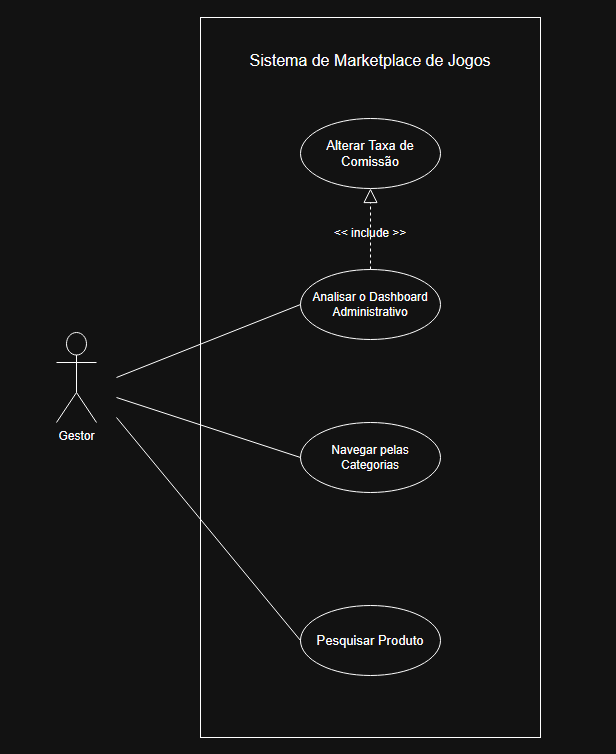
\includegraphics[width=0.9\textwidth]{images/image7.png}
  \caption{Diagrama de casos de uso do gestor}
  \label{fig:usecase-gestor}
  \legend{Fonte: Autor (2026).}
\end{figure}

\begin{figure}[htbp]
  \centering
  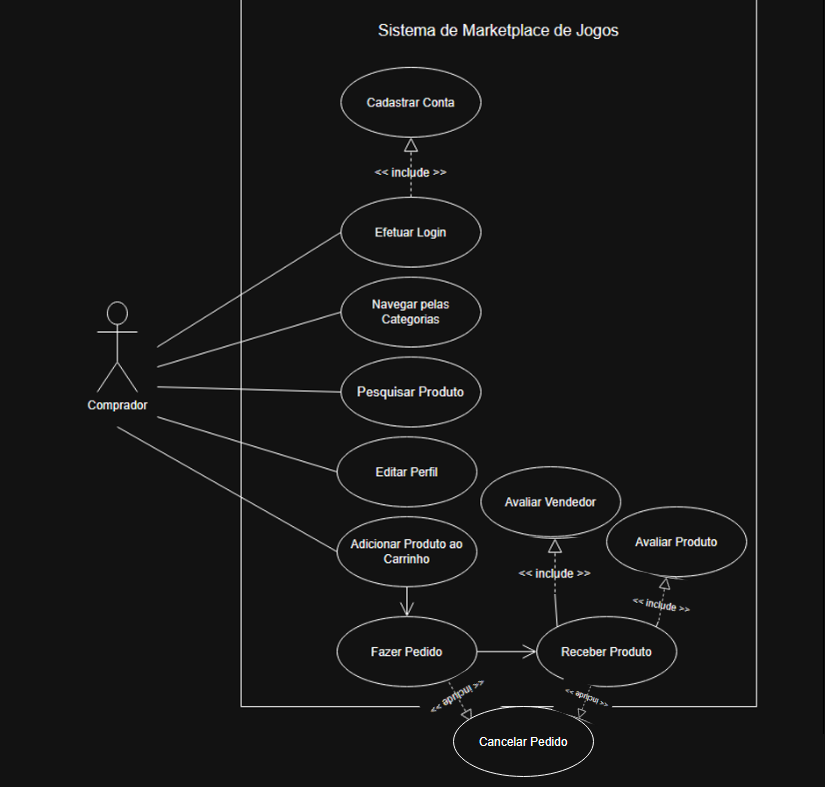
\includegraphics[width=0.9\textwidth]{images/image8.png}
  \caption{Diagrama de casos de uso do comprador}
  \label{fig:usecase-comprador}
  \legend{Fonte: Autor (2026).}
\end{figure}

\begin{figure}[htbp]
  \centering
  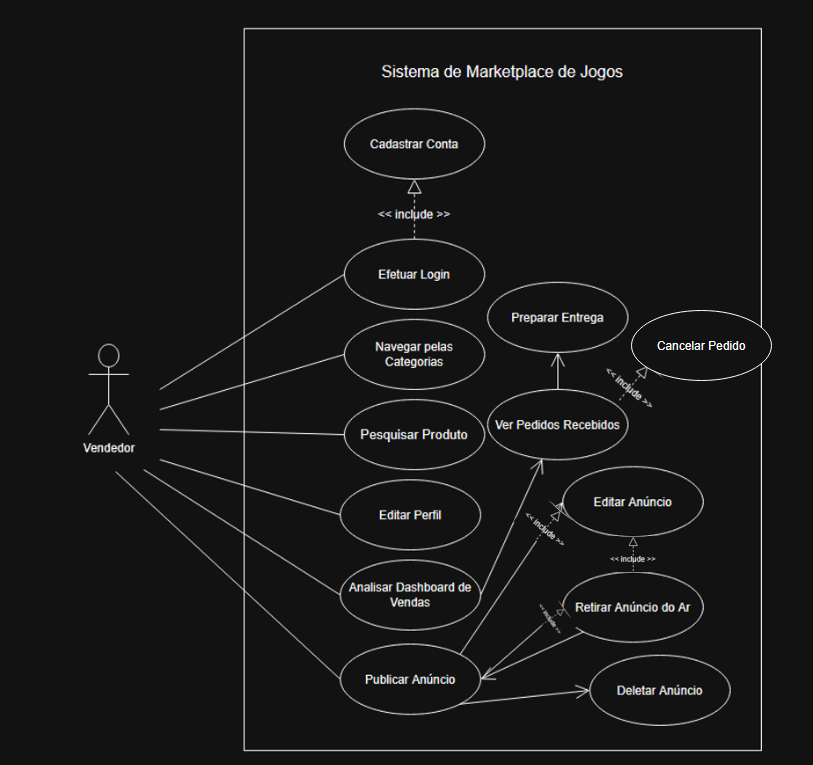
\includegraphics[width=0.9\textwidth]{images/image9.png}
  \caption{Diagrama de casos de uso do vendedor}
  \label{fig:usecase-vendedor}
  \legend{Fonte: Autor (2026).}
\end{figure}

\subsection{Descrições de casos de uso}

Estes são os casos de uso mostrados na subseção anterior, porém sob uma
perspectiva individual e detalhada.

{\captionsetup{name=Quadro}
\begin{longtable}[]{@{}
  >{\raggedright\arraybackslash}p{(\linewidth - 2\tabcolsep) * \real{0.5000}}
  >{\raggedright\arraybackslash}p{(\linewidth - 2\tabcolsep) * \real{0.5000}}@{}}
\caption{Cadastrar conta}\label{qua:cadastrar-conta}\\
\toprule\noalign{}
\begin{minipage}[b]{\linewidth}\centering
\textbf{Nome do Caso de Uso}
\end{minipage} & \begin{minipage}[b]{\linewidth}\raggedright
Cadastrar Conta
\end{minipage} \\
\midrule\noalign{}
\endfirsthead
\toprule\noalign{}
\begin{minipage}[b]{\linewidth}\centering
\textbf{Nome do Caso de Uso}
\end{minipage} & \begin{minipage}[b]{\linewidth}\raggedright
Cadastrar Conta
\end{minipage} \\
\midrule\noalign{}
\endhead
\bottomrule\noalign{}
\endlastfoot
\textbf{Ator Principal} & Vendedor; Comprador \\
\textbf{Ator Secundário} & \\
\textbf{Resumo} & Cadastrar uma nova conta de usuário no sistema. \\
\textbf{Pré-Condições} & \\
\textbf{Pós-Condições} & Efetuar Login \\
\end{longtable}
\legend{Fonte: Autor (2026).}
}

{\captionsetup{name=Quadro}
\begin{longtable}[]{@{}
  >{\raggedright\arraybackslash}p{(\linewidth - 2\tabcolsep) * \real{0.5000}}
  >{\raggedright\arraybackslash}p{(\linewidth - 2\tabcolsep) * \real{0.5000}}@{}}
\caption{Efetuar login}\label{qua:efetuar-login}\\
\toprule\noalign{}
\begin{minipage}[b]{\linewidth}\centering
\textbf{Nome do Caso de Uso}
\end{minipage} & \begin{minipage}[b]{\linewidth}\raggedright
Efetuar Login
\end{minipage} \\
\midrule\noalign{}
\endfirsthead
\toprule\noalign{}
\begin{minipage}[b]{\linewidth}\centering
\textbf{Nome do Caso de Uso}
\end{minipage} & \begin{minipage}[b]{\linewidth}\raggedright
Efetuar Login
\end{minipage} \\
\midrule\noalign{}
\endhead
\bottomrule\noalign{}
\endlastfoot
\textbf{Ator Principal} & Comprador; Vendedor \\
\textbf{Ator Secundário} & \\
\textbf{Resumo} & Efetuar login em uma conta de usuário cadastrada no
sistema. \\
\textbf{Pré-Condições} & Cadastrar Conta \\
\textbf{Pós-Condições} & \\
\end{longtable}
\legend{Fonte: Autor (2026).}
}

{\captionsetup{name=Quadro}
\begin{longtable}[]{@{}
  >{\raggedright\arraybackslash}p{(\linewidth - 2\tabcolsep) * \real{0.5000}}
  >{\raggedright\arraybackslash}p{(\linewidth - 2\tabcolsep) * \real{0.5000}}@{}}
\caption{Navegar pelas categorias}\label{qua:navegar-categorias}\\
\toprule\noalign{}
\begin{minipage}[b]{\linewidth}\centering
\textbf{Nome do Caso de Uso}
\end{minipage} & \begin{minipage}[b]{\linewidth}\raggedright
Navegar pelas Categorias
\end{minipage} \\
\midrule\noalign{}
\endfirsthead
\toprule\noalign{}
\begin{minipage}[b]{\linewidth}\centering
\textbf{Nome do Caso de Uso}
\end{minipage} & \begin{minipage}[b]{\linewidth}\raggedright
Navegar pelas Categorias
\end{minipage} \\
\midrule\noalign{}
\endhead
\bottomrule\noalign{}
\endlastfoot
\textbf{Ator Principal} & Gestor; Comprador; Vendedor \\
\textbf{Ator Secundário} & \\
\textbf{Resumo} & Navegar pela aba de ``Categorias'' e ver os diferentes
produtos de cada categoria. \\
\textbf{Pré-Condições} & \\
\textbf{Pós-Condições} & \\
\end{longtable}
\legend{Fonte: Autor (2026).}
}

{\captionsetup{name=Quadro}
\begin{longtable}[]{@{}
  >{\raggedright\arraybackslash}p{(\linewidth - 2\tabcolsep) * \real{0.5000}}
  >{\raggedright\arraybackslash}p{(\linewidth - 2\tabcolsep) * \real{0.5000}}@{}}
\caption{Pesquisar produto}\label{qua:pesquisar-produto}\\
\toprule\noalign{}
\begin{minipage}[b]{\linewidth}\centering
\textbf{Nome do Caso de Uso}
\end{minipage} & \begin{minipage}[b]{\linewidth}\raggedright
Pesquisar Produto
\end{minipage} \\
\midrule\noalign{}
\endfirsthead
\toprule\noalign{}
\begin{minipage}[b]{\linewidth}\centering
\textbf{Nome do Caso de Uso}
\end{minipage} & \begin{minipage}[b]{\linewidth}\raggedright
Pesquisar Produto
\end{minipage} \\
\midrule\noalign{}
\endhead
\bottomrule\noalign{}
\endlastfoot
\textbf{Ator Principal} & Gestor; Vendedor; Comprador \\
\textbf{Ator Secundário} & \\
\textbf{Resumo} & Pesquisar um produto na barra de busca do sistema. \\
\textbf{Pré-Condições} & \\
\textbf{Pós-Condições} & \\
\end{longtable}
\legend{Fonte: Autor (2026).}
}

{\captionsetup{name=Quadro}
\begin{longtable}[]{@{}
  >{\raggedright\arraybackslash}p{(\linewidth - 2\tabcolsep) * \real{0.5000}}
  >{\raggedright\arraybackslash}p{(\linewidth - 2\tabcolsep) * \real{0.5000}}@{}}
\caption{Editar perfil}\label{qua:editar-perfil}\\
\toprule\noalign{}
\begin{minipage}[b]{\linewidth}\centering
\textbf{Nome do Caso de Uso}
\end{minipage} & \begin{minipage}[b]{\linewidth}\raggedright
Editar Perfil
\end{minipage} \\
\midrule\noalign{}
\endfirsthead
\toprule\noalign{}
\begin{minipage}[b]{\linewidth}\centering
\textbf{Nome do Caso de Uso}
\end{minipage} & \begin{minipage}[b]{\linewidth}\raggedright
Editar Perfil
\end{minipage} \\
\midrule\noalign{}
\endhead
\bottomrule\noalign{}
\endlastfoot
\textbf{Ator Principal} & Vendedor; Comprador \\
\textbf{Ator Secundário} & \\
\textbf{Resumo} & Editar as informações inseridas no perfil (nome,
senha, localização...) \\
\textbf{Pré-Condições} & \\
\textbf{Pós-Condições} & \\
\end{longtable}
\legend{Fonte: Autor (2026).}
}

{\captionsetup{name=Quadro}
\begin{longtable}[]{@{}
  >{\raggedright\arraybackslash}p{(\linewidth - 2\tabcolsep) * \real{0.5000}}
  >{\raggedright\arraybackslash}p{(\linewidth - 2\tabcolsep) * \real{0.5000}}@{}}
\caption{Analisar o \emph{dashboard} administrativo}\label{qua:dashboard-adm}\\
\toprule\noalign{}
\begin{minipage}[b]{\linewidth}\centering
\textbf{Nome do Caso de Uso}
\end{minipage} & \begin{minipage}[b]{\linewidth}\raggedright
Analisar o Dashboard Administrativo
\end{minipage} \\
\midrule\noalign{}
\endfirsthead
\toprule\noalign{}
\begin{minipage}[b]{\linewidth}\centering
\textbf{Nome do Caso de Uso}
\end{minipage} & \begin{minipage}[b]{\linewidth}\raggedright
Analisar o Dashboard Administrativo
\end{minipage} \\
\midrule\noalign{}
\endhead
\bottomrule\noalign{}
\endlastfoot
\textbf{Ator Principal} & Gestor \\
\textbf{Ator Secundário} & \\
\textbf{Resumo} & Observar o painel administrativo para ver os
relatórios do sistema e estatísticas de venda. \\
\textbf{Pré-Condições} & \\
\textbf{Pós-Condições} & Alterar a Taxa de Comissão \\
\end{longtable}
\legend{Fonte: Autor (2026).}
}

{\captionsetup{name=Quadro}
\begin{longtable}[]{@{}
  >{\raggedright\arraybackslash}p{(\linewidth - 2\tabcolsep) * \real{0.5000}}
  >{\raggedright\arraybackslash}p{(\linewidth - 2\tabcolsep) * \real{0.5000}}@{}}
\caption{Alterar taxa de comissão}\label{qua:alterar-comissao}\\
\toprule\noalign{}
\begin{minipage}[b]{\linewidth}\centering
\textbf{Nome do Caso de Uso}
\end{minipage} & \begin{minipage}[b]{\linewidth}\raggedright
Alterar Taxa de Comissão
\end{minipage} \\
\midrule\noalign{}
\endfirsthead
\toprule\noalign{}
\begin{minipage}[b]{\linewidth}\centering
\textbf{Nome do Caso de Uso}
\end{minipage} & \begin{minipage}[b]{\linewidth}\raggedright
Alterar Taxa de Comissão
\end{minipage} \\
\midrule\noalign{}
\endhead
\bottomrule\noalign{}
\endlastfoot
\textbf{Ator Principal} & Gestor \\
\textbf{Ator Secundário} & \\
\textbf{Resumo} & Alterar a taxa da comissão obtida através das
transações. \\
\textbf{Pré-Condições} & Analisar o Dashboard Administrativo \\
\textbf{Pós-Condições} & \\
\end{longtable}
\legend{Fonte: Autor (2026).}
}

{\captionsetup{name=Quadro}
\begin{longtable}[]{@{}
  >{\raggedright\arraybackslash}p{(\linewidth - 2\tabcolsep) * \real{0.5000}}
  >{\raggedright\arraybackslash}p{(\linewidth - 2\tabcolsep) * \real{0.5000}}@{}}
\caption{Adicionar produto ao carrinho}\label{qua:add-carrinho}\\
\toprule\noalign{}
\begin{minipage}[b]{\linewidth}\centering
\textbf{Nome do Caso de Uso}
\end{minipage} & \begin{minipage}[b]{\linewidth}\raggedright
Adicionar Produto ao Carrinho
\end{minipage} \\
\midrule\noalign{}
\endfirsthead
\toprule\noalign{}
\begin{minipage}[b]{\linewidth}\centering
\textbf{Nome do Caso de Uso}
\end{minipage} & \begin{minipage}[b]{\linewidth}\raggedright
Adicionar Produto ao Carrinho
\end{minipage} \\
\midrule\noalign{}
\endhead
\bottomrule\noalign{}
\endlastfoot
\textbf{Ator Principal} & Comprador \\
\textbf{Ator Secundário} & \\
\textbf{Resumo} & O comprador adiciona um produto que gostaria de
comprar ao seu carrinho. \\
\textbf{Pré-Condições} & \\
\textbf{Pós-Condições} & Fazer Pedido \\
\end{longtable}
\legend{Fonte: Autor (2026).}
}

{\captionsetup{name=Quadro}
\begin{longtable}[]{@{}
  >{\raggedright\arraybackslash}p{(\linewidth - 2\tabcolsep) * \real{0.5000}}
  >{\raggedright\arraybackslash}p{(\linewidth - 2\tabcolsep) * \real{0.5000}}@{}}
\caption{Fazer pedido}\label{qua:fazer-pedido}\\
\toprule\noalign{}
\begin{minipage}[b]{\linewidth}\centering
\textbf{Nome do Caso de Uso}
\end{minipage} & \begin{minipage}[b]{\linewidth}\raggedright
Fazer Pedido
\end{minipage} \\
\midrule\noalign{}
\endfirsthead
\toprule\noalign{}
\begin{minipage}[b]{\linewidth}\centering
\textbf{Nome do Caso de Uso}
\end{minipage} & \begin{minipage}[b]{\linewidth}\raggedright
Fazer Pedido
\end{minipage} \\
\midrule\noalign{}
\endhead
\bottomrule\noalign{}
\endlastfoot
\textbf{Ator Principal} & Comprador \\
\textbf{Ator Secundário} & \\
\textbf{Resumo} & O usuário finaliza o pedido com todos os itens
presentes em seu carrinho. \\
\textbf{Pré-Condições} & Adicionar Produto ao Carrinho \\
\textbf{Pós-Condições} & Cancelar Pedido; Receber Produto \\
\end{longtable}
\legend{Fonte: Autor (2026).}
}

{\captionsetup{name=Quadro}
\begin{longtable}[]{@{}
  >{\raggedright\arraybackslash}p{(\linewidth - 2\tabcolsep) * \real{0.5000}}
  >{\raggedright\arraybackslash}p{(\linewidth - 2\tabcolsep) * \real{0.5000}}@{}}
\caption{Receber produto}\label{qua:receber-produto}\\
\toprule\noalign{}
\begin{minipage}[b]{\linewidth}\centering
\textbf{Nome do Caso de Uso}
\end{minipage} & \begin{minipage}[b]{\linewidth}\raggedright
Receber Produto
\end{minipage} \\
\midrule\noalign{}
\endfirsthead
\toprule\noalign{}
\begin{minipage}[b]{\linewidth}\centering
\textbf{Nome do Caso de Uso}
\end{minipage} & \begin{minipage}[b]{\linewidth}\raggedright
Receber Produto
\end{minipage} \\
\midrule\noalign{}
\endhead
\bottomrule\noalign{}
\endlastfoot
\textbf{Ator Principal} & Comprador \\
\textbf{Ator Secundário} & Vendedor \\
\textbf{Resumo} & Após a preparação da entrega, o comprador recebe o
produto. \\
\textbf{Pré-Condições} & Fazer Pedido \\
\textbf{Pós-Condições} & Cancelar Pedido; Avaliar Vendedor; Avaliar
Produto \\
\end{longtable}
\legend{Fonte: Autor (2026).}
}

{\captionsetup{name=Quadro}
\begin{longtable}[]{@{}
  >{\raggedright\arraybackslash}p{(\linewidth - 2\tabcolsep) * \real{0.5000}}
  >{\raggedright\arraybackslash}p{(\linewidth - 2\tabcolsep) * \real{0.5000}}@{}}
\caption{Avaliar vendedor}\label{qua:avaliar-vendedor}\\
\toprule\noalign{}
\begin{minipage}[b]{\linewidth}\centering
\textbf{Nome do Caso de Uso}
\end{minipage} & \begin{minipage}[b]{\linewidth}\raggedright
Avaliar Vendedor
\end{minipage} \\
\midrule\noalign{}
\endfirsthead
\toprule\noalign{}
\begin{minipage}[b]{\linewidth}\centering
\textbf{Nome do Caso de Uso}
\end{minipage} & \begin{minipage}[b]{\linewidth}\raggedright
Avaliar Vendedor
\end{minipage} \\
\midrule\noalign{}
\endhead
\bottomrule\noalign{}
\endlastfoot
\textbf{Ator Principal} & Comprador \\
\textbf{Ator Secundário} & \\
\textbf{Resumo} & Após receber um produto que comprou, o usuário avalia
o vendedor. \\
\textbf{Pré-Condições} & Receber Produto \\
\textbf{Pós-Condições} & \\
\end{longtable}
\legend{Fonte: Autor (2026).}
}

{\captionsetup{name=Quadro}
\begin{longtable}[]{@{}
  >{\raggedright\arraybackslash}p{(\linewidth - 2\tabcolsep) * \real{0.5000}}
  >{\raggedright\arraybackslash}p{(\linewidth - 2\tabcolsep) * \real{0.5000}}@{}}
\caption{Avaliar produto}\label{qua:avaliar-produto}\\
\toprule\noalign{}
\begin{minipage}[b]{\linewidth}\centering
\textbf{Nome do Caso de Uso}
\end{minipage} & \begin{minipage}[b]{\linewidth}\raggedright
Avaliar Produto
\end{minipage} \\
\midrule\noalign{}
\endfirsthead
\toprule\noalign{}
\begin{minipage}[b]{\linewidth}\centering
\textbf{Nome do Caso de Uso}
\end{minipage} & \begin{minipage}[b]{\linewidth}\raggedright
Avaliar Produto
\end{minipage} \\
\midrule\noalign{}
\endhead
\bottomrule\noalign{}
\endlastfoot
\textbf{Ator Principal} & Comprador \\
\textbf{Ator Secundário} & \\
\textbf{Resumo} & O usuário avalia um produto que comprou após
recebê-lo. \\
\textbf{Pré-Condições} & Receber Produto \\
\textbf{Pós-Condições} & \\
\end{longtable}
\legend{Fonte: Autor (2026).}
}

{\captionsetup{name=Quadro}
\begin{longtable}[]{@{}
  >{\raggedright\arraybackslash}p{(\linewidth - 2\tabcolsep) * \real{0.5000}}
  >{\raggedright\arraybackslash}p{(\linewidth - 2\tabcolsep) * \real{0.5000}}@{}}
\caption{Cancelar pedido}\label{qua:cancelar-pedido}\\
\toprule\noalign{}
\begin{minipage}[b]{\linewidth}\centering
\textbf{Nome do Caso de Uso}
\end{minipage} & \begin{minipage}[b]{\linewidth}\raggedright
Cancelar Pedido
\end{minipage} \\
\midrule\noalign{}
\endfirsthead
\toprule\noalign{}
\begin{minipage}[b]{\linewidth}\centering
\textbf{Nome do Caso de Uso}
\end{minipage} & \begin{minipage}[b]{\linewidth}\raggedright
Cancelar Pedido
\end{minipage} \\
\midrule\noalign{}
\endhead
\bottomrule\noalign{}
\endlastfoot
\textbf{Ator Principal} & Comprador; Vendedor \\
\textbf{Ator Secundário} & \\
\textbf{Resumo} & O pedido é cancelado, seja pelo comprador ou pelo
vendedor. Isso pode inclusive ser feito após a entrega do produto, por
um determinado período. \\
\textbf{Pré-Condições} & Fazer Pedido; Receber Produto; Ver Produtos
Recebidos \\
\textbf{Pós-Condições} & \\
\end{longtable}
\legend{Fonte: Autor (2026).}
}

{\captionsetup{name=Quadro}
\begin{longtable}[]{@{}
  >{\raggedright\arraybackslash}p{(\linewidth - 2\tabcolsep) * \real{0.5000}}
  >{\raggedright\arraybackslash}p{(\linewidth - 2\tabcolsep) * \real{0.5000}}@{}}
\caption{Analisar \emph{dashboard} de vendas}\label{qua:dashboard-vendas}\\
\toprule\noalign{}
\begin{minipage}[b]{\linewidth}\centering
\textbf{Nome do Caso de Uso}
\end{minipage} & \begin{minipage}[b]{\linewidth}\raggedright
Analisar Dashboard de Vendas
\end{minipage} \\
\midrule\noalign{}
\endfirsthead
\toprule\noalign{}
\begin{minipage}[b]{\linewidth}\centering
\textbf{Nome do Caso de Uso}
\end{minipage} & \begin{minipage}[b]{\linewidth}\raggedright
Analisar Dashboard de Vendas
\end{minipage} \\
\midrule\noalign{}
\endhead
\bottomrule\noalign{}
\endlastfoot
\textbf{Ator Principal} & Vendedor \\
\textbf{Ator Secundário} & \\
\textbf{Resumo} & O vendedor analisa seu dashboard de vendas para ver
suas estatísticas e relatórios. \\
\textbf{Pré-Condições} & \\
\textbf{Pós-Condições} & Ver Pedidos Recebidos \\
\end{longtable}
\legend{Fonte: Autor (2026).}
}

{\captionsetup{name=Quadro}
\begin{longtable}[]{@{}
  >{\raggedright\arraybackslash}p{(\linewidth - 2\tabcolsep) * \real{0.5000}}
  >{\raggedright\arraybackslash}p{(\linewidth - 2\tabcolsep) * \real{0.5000}}@{}}
\caption{Ver pedidos recebidos}\label{qua:ver-pedidos-recebidos}\\
\toprule\noalign{}
\begin{minipage}[b]{\linewidth}\centering
\textbf{Nome do Caso de Uso}
\end{minipage} & \begin{minipage}[b]{\linewidth}\raggedright
Ver Pedidos Recebidos
\end{minipage} \\
\midrule\noalign{}
\endfirsthead
\toprule\noalign{}
\begin{minipage}[b]{\linewidth}\centering
\textbf{Nome do Caso de Uso}
\end{minipage} & \begin{minipage}[b]{\linewidth}\raggedright
Ver Pedidos Recebidos
\end{minipage} \\
\midrule\noalign{}
\endhead
\bottomrule\noalign{}
\endlastfoot
\textbf{Ator Principal} & Vendedor \\
\textbf{Ator Secundário} & \\
\textbf{Resumo} & O vendedor vê os pedidos que recebeu de
compradores. \\
\textbf{Pré-Condições} & Analisar Dashboard de Vendas \\
\textbf{Pós-Condições} & Cancelar Pedido; Preparar Entrega \\
\end{longtable}
\legend{Fonte: Autor (2026).}
}

{\captionsetup{name=Quadro}
\begin{longtable}[]{@{}
  >{\raggedright\arraybackslash}p{(\linewidth - 2\tabcolsep) * \real{0.5000}}
  >{\raggedright\arraybackslash}p{(\linewidth - 2\tabcolsep) * \real{0.5000}}@{}}
\caption{Preparar entrega}\label{qua:preparar-entrega}\\
\toprule\noalign{}
\begin{minipage}[b]{\linewidth}\centering
\textbf{Nome do Caso de Uso}
\end{minipage} & \begin{minipage}[b]{\linewidth}\raggedright
Preparar Entrega
\end{minipage} \\
\midrule\noalign{}
\endfirsthead
\toprule\noalign{}
\begin{minipage}[b]{\linewidth}\centering
\textbf{Nome do Caso de Uso}
\end{minipage} & \begin{minipage}[b]{\linewidth}\raggedright
Preparar Entrega
\end{minipage} \\
\midrule\noalign{}
\endhead
\bottomrule\noalign{}
\endlastfoot
\textbf{Ator Principal} & Vendedor \\
\textbf{Ator Secundário} & \\
\textbf{Resumo} & O vendedor prepara a entrega de um produto para o
comprador. \\
\textbf{Pré-Condições} & Ver Pedidos Recebidos \\
\textbf{Pós-Condições} & \\
\end{longtable}
\legend{Fonte: Autor (2026).}
}

{\captionsetup{name=Quadro}
\begin{longtable}[]{@{}
  >{\raggedright\arraybackslash}p{(\linewidth - 2\tabcolsep) * \real{0.5000}}
  >{\raggedright\arraybackslash}p{(\linewidth - 2\tabcolsep) * \real{0.5000}}@{}}
\caption{Publicar anúncio}\label{qua:publicar-anuncio}\\
\toprule\noalign{}
\begin{minipage}[b]{\linewidth}\centering
\textbf{Nome do Caso de Uso}
\end{minipage} & \begin{minipage}[b]{\linewidth}\raggedright
Publicar Anúncio
\end{minipage} \\
\midrule\noalign{}
\endfirsthead
\toprule\noalign{}
\begin{minipage}[b]{\linewidth}\centering
\textbf{Nome do Caso de Uso}
\end{minipage} & \begin{minipage}[b]{\linewidth}\raggedright
Publicar Anúncio
\end{minipage} \\
\midrule\noalign{}
\endhead
\bottomrule\noalign{}
\endlastfoot
\textbf{Ator Principal} & Vendedor \\
\textbf{Ator Secundário} & \\
\textbf{Resumo} & O vendedor publica o anúncio de um produto para
vendê-lo. \\
\textbf{Pré-Condições} & Retirar Anúncio do Ar \\
\textbf{Pós-Condições} & Retirar Anúncio do Ar; Editar Anúncio \\
\end{longtable}
\legend{Fonte: Autor (2026).}
}

{\captionsetup{name=Quadro}
\begin{longtable}[]{@{}
  >{\raggedright\arraybackslash}p{(\linewidth - 2\tabcolsep) * \real{0.5000}}
  >{\raggedright\arraybackslash}p{(\linewidth - 2\tabcolsep) * \real{0.5000}}@{}}
\caption{Editar anúncio}\label{qua:editar-anuncio}\\
\toprule\noalign{}
\begin{minipage}[b]{\linewidth}\centering
\textbf{Nome do Caso de Uso}
\end{minipage} & \begin{minipage}[b]{\linewidth}\raggedright
Editar Anúncio
\end{minipage} \\
\midrule\noalign{}
\endfirsthead
\toprule\noalign{}
\begin{minipage}[b]{\linewidth}\centering
\textbf{Nome do Caso de Uso}
\end{minipage} & \begin{minipage}[b]{\linewidth}\raggedright
Editar Anúncio
\end{minipage} \\
\midrule\noalign{}
\endhead
\bottomrule\noalign{}
\endlastfoot
\textbf{Ator Principal} & Vendedor \\
\textbf{Ator Secundário} & \\
\textbf{Resumo} & O vendedor edita as informações de um anúncio após sua
publicação inicial. \\
\textbf{Pré-Condições} & Publicar Anúncio \\
\textbf{Pós-Condições} & \\
\end{longtable}
\legend{Fonte: Autor (2026).}
}

{\captionsetup{name=Quadro}
\begin{longtable}[]{@{}
  >{\raggedright\arraybackslash}p{(\linewidth - 2\tabcolsep) * \real{0.5000}}
  >{\raggedright\arraybackslash}p{(\linewidth - 2\tabcolsep) * \real{0.5000}}@{}}
\caption{Retirar anúncio do ar}\label{qua:retirar-anuncio}\\
\toprule\noalign{}
\begin{minipage}[b]{\linewidth}\centering
\textbf{Nome do Caso de Uso}
\end{minipage} & \begin{minipage}[b]{\linewidth}\raggedright
Retirar Anúncio do Ar
\end{minipage} \\
\midrule\noalign{}
\endfirsthead
\toprule\noalign{}
\begin{minipage}[b]{\linewidth}\centering
\textbf{Nome do Caso de Uso}
\end{minipage} & \begin{minipage}[b]{\linewidth}\raggedright
Retirar Anúncio do Ar
\end{minipage} \\
\midrule\noalign{}
\endhead
\bottomrule\noalign{}
\endlastfoot
\textbf{Ator Principal} & Vendedor \\
\textbf{Ator Secundário} & \\
\textbf{Resumo} & O vendedor retira o anúncio do ar temporariamente.
Ele pode ainda editá-lo nesse estado. \\
\textbf{Pré-Condições} & Publicar Anúncio \\
\textbf{Pós-Condições} & Publicar Anúncio; Editar Anúncio \\
\end{longtable}
\legend{Fonte: Autor (2026).}
}

{\captionsetup{name=Quadro}
\begin{longtable}[]{@{}
  >{\raggedright\arraybackslash}p{(\linewidth - 2\tabcolsep) * \real{0.5000}}
  >{\raggedright\arraybackslash}p{(\linewidth - 2\tabcolsep) * \real{0.5000}}@{}}
\caption{Deletar anúncio}\label{qua:deletar-anuncio}\\
\toprule\noalign{}
\begin{minipage}[b]{\linewidth}\centering
\textbf{Nome do Caso de Uso}
\end{minipage} & \begin{minipage}[b]{\linewidth}\raggedright
Deletar Anúncio
\end{minipage} \\
\midrule\noalign{}
\endfirsthead
\toprule\noalign{}
\begin{minipage}[b]{\linewidth}\centering
\textbf{Nome do Caso de Uso}
\end{minipage} & \begin{minipage}[b]{\linewidth}\raggedright
Deletar Anúncio
\end{minipage} \\
\midrule\noalign{}
\endhead
\bottomrule\noalign{}
\endlastfoot
\textbf{Ator Principal} & Vendedor \\
\textbf{Ator Secundário} & \\
\textbf{Resumo} & O vendedor deleta um anúncio (ao menos para si e
outros usuários comuns; os registros ainda ficarão no sistema por
garantia). \\
\textbf{Pré-Condições} & Publicar Anúncio \\
\textbf{Pós-Condições} & \\
\end{longtable}
\legend{Fonte: Autor (2026).}
}

\section{Arquitetura}

A arquitetura do sistema é dividida em diversos componentes, como é
padrão do Django. As imagens mostram as pastas específicas em maiores
detalhes, sendo que todos os componentes possuem os mesmos
arquivos-base, exceto por core (o ``núcleo'', que é padrão na criação de
um novo projeto, ao invés de ser criado pelo desenvolvedor).

\begin{figure}[htbp]
  \centering
  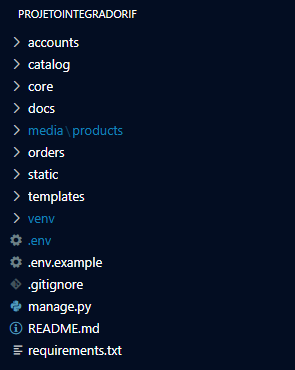
\includegraphics[width=0.75\textwidth]{images/image10.png}
  \caption{Estrutura de arquivos geral do projeto}
  \label{fig:estrutura-geral}
  \legend{Fonte: Autor (2026).}
\end{figure}

\begin{figure}[htbp]
  \centering
  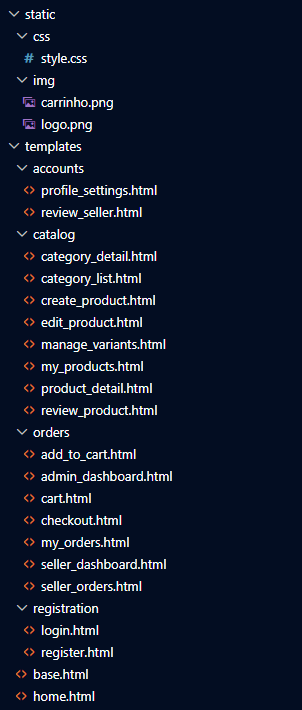
\includegraphics[width=0.6\textwidth]{images/image11.png}
  \caption{Detalhamento da estrutura de arquivos \#1}
  \label{fig:estrutura-detalhe-1}
  \legend{Fonte: Autor (2026).}
\end{figure}

\begin{figure}[htbp]
  \centering
  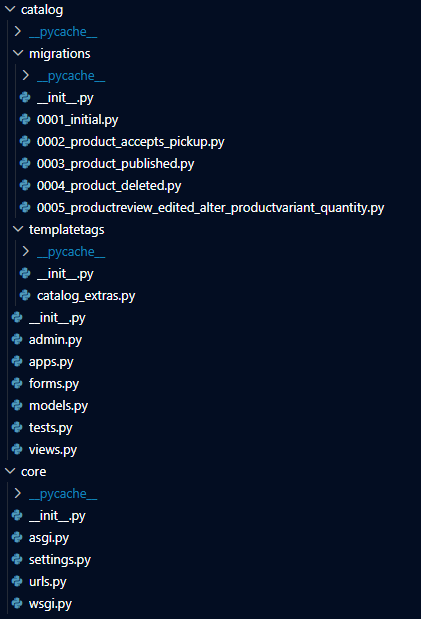
\includegraphics[width=0.75\textwidth]{images/image12.png}
  \caption{Detalhamento da estrutura de arquivos \#2}
  \label{fig:estrutura-detalhe-2}
  \legend{Fonte: Autor (2026).}
\end{figure}

\section{Projeto de dados}

A principal fonte acadêmica a respeito do tema ``banco de dados'' é
Coronel e suas obras, com vários coautores ao decorrer dos anos, tais
como Morris e Rob. \citeonline[p. 37]{morris2016sbd} afirmam, acerca do design de
dados que forma a base de um projeto:

\begin{quote}
Design de banco de dados se refere às atividades que focam no design da
estrutura do banco de dados que será utilizada para armazenar e
gerenciar dados de usuários do sistema. Um banco de dados que cumpre
todos os requisitos de usuário não surge por mágica; sua estrutura deve
ser planejada cuidadosamente. {[}...{]} Até um SGBD bom terá uma
performance ruim com um banco de dados de design ruim.
\end{quote}

Sendo assim, o Supabase foi escolhido para se alinhar com esses
princípios. Através de sua integração com o Django para viabilizar o
processo de \emph{migration}, e de sua interface \emph{web} intuitiva,
ele permite conveniência e rapidez na gestão do design de banco de
dados, sendo que ele automaticamente cria um diagrama
entidade-relacionamento (DER) de todo o banco e também possui um editor
SQL embutido caso precisem ser feitas mudanças espontâneas.
\begin{figure}[htbp]
  \centering
  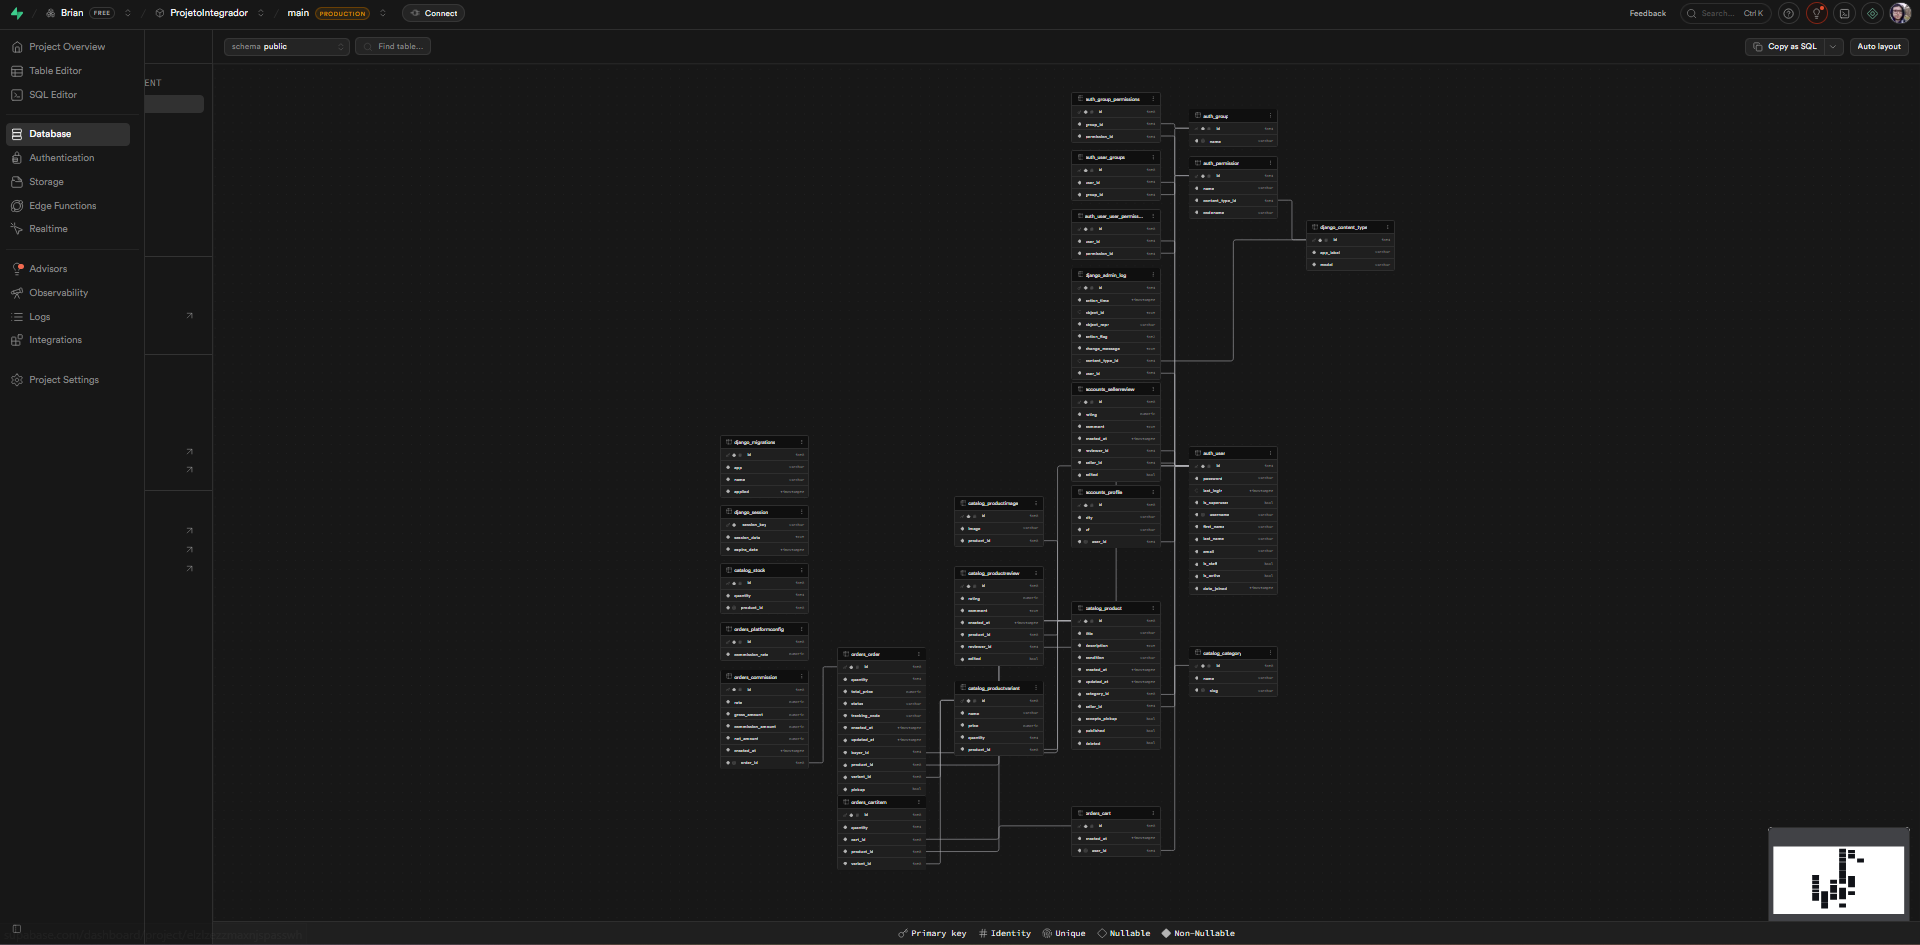
\includegraphics[width=0.95\textwidth]{images/image13.png}
  \caption{DER do banco de dados}
  \label{fig:der-bd}
  \legend{Fonte: Autor (2026).}
\end{figure}


\subsection{Dicionário de dados}

Aqui, serão apresentados os dicionários de dados das tabelas relevantes
ao projeto (tendo em mente que muitas das tabelas vistas no DER acima
são componentes padrão do Django).

{\captionsetup{name=Quadro}
\begin{longtable}[]{@{}
  >{\centering\arraybackslash}p{(\linewidth - 8\tabcolsep) * \real{0.1765}}
  >{\centering\arraybackslash}p{(\linewidth - 8\tabcolsep) * \real{0.2941}}
  >{\centering\arraybackslash}p{(\linewidth - 8\tabcolsep) * \real{0.1765}}
  >{\raggedright\arraybackslash}p{(\linewidth - 8\tabcolsep) * \real{0.2353}}
  >{\raggedright\arraybackslash}p{(\linewidth - 8\tabcolsep) * \real{0.1176}}@{}}
\caption{Usuários}\label{qua:usuarios}\\
\toprule\noalign{}
\multicolumn{5}{@{}>{\centering\arraybackslash}p{(\linewidth - 8\tabcolsep) * \real{1.0000} + 8\tabcolsep}@{}}{%
\begin{minipage}[b]{\linewidth}\centering
\textbf{Tabela de Usuários}
\end{minipage}} \\
\midrule\noalign{}
\endfirsthead
\toprule\noalign{}
\multicolumn{5}{@{}>{\centering\arraybackslash}p{(\linewidth - 8\tabcolsep) * \real{1.0000} + 8\tabcolsep}@{}}{%
\begin{minipage}[b]{\linewidth}\centering
\textbf{Tabela de Usuários}
\end{minipage}} \\
\midrule\noalign{}
\endhead
\bottomrule\noalign{}
\endlastfoot
\textbf{Nome} & \textbf{Conteúdo} & \textbf{Tipo} &
\textbf{Obrigatoriedade} & \textbf{Chave?} \\
id & ID do usuário & int4 & SIM & PK \\
password & Senha do usuário & varchar & SIM & \\
last\_login & Data do último login do usuário & timestamptz & SIM & \\
is\_superuser & O usuário é um superusuário do sistema? & bool & SIM
& \\
username & Nome do usuário dentro da plataforma & varchar & SIM & \\
first\_name & Nome real do usuário & varchar & SIM & \\
last\_name & Sobrenome do usuário & varchar & SIM & \\
email & Email do usuário & varchar & SIM & \\
is\_staff & O usuário faz parte da equipe por trás do sistema? & bool &
SIM & \\
is\_active & O usuário é ativo? & bool & SIM & \\
date\_joined & Data na qual o usuário criou sua conta & timestamptz &
SIM & \\
\end{longtable}
\legend{Fonte: Autor (2026).}
}

{\captionsetup{name=Quadro}
\begin{longtable}[]{@{}
  >{\centering\arraybackslash}p{(\linewidth - 8\tabcolsep) * \real{0.1765}}
  >{\centering\arraybackslash}p{(\linewidth - 8\tabcolsep) * \real{0.3530}}
  >{\centering\arraybackslash}p{(\linewidth - 8\tabcolsep) * \real{0.1176}}
  >{\raggedright\arraybackslash}p{(\linewidth - 8\tabcolsep) * \real{0.2352}}
  >{\raggedright\arraybackslash}p{(\linewidth - 8\tabcolsep) * \real{0.1176}}@{}}
\caption{Categorias}\label{qua:categorias-dd}\\
\toprule\noalign{}
\multicolumn{5}{@{}>{\centering\arraybackslash}p{(\linewidth - 8\tabcolsep) * \real{1.0000} + 8\tabcolsep}@{}}{%
\begin{minipage}[b]{\linewidth}\centering
\textbf{Tabela de Categorias}
\end{minipage}} \\
\midrule\noalign{}
\endfirsthead
\toprule\noalign{}
\multicolumn{5}{@{}>{\centering\arraybackslash}p{(\linewidth - 8\tabcolsep) * \real{1.0000} + 8\tabcolsep}@{}}{%
\begin{minipage}[b]{\linewidth}\centering
\textbf{Tabela de Categorias}
\end{minipage}} \\
\midrule\noalign{}
\endhead
\bottomrule\noalign{}
\endlastfoot
\textbf{Nome} & \textbf{Conteúdo} & \textbf{Tipo} &
\textbf{Obrigatoriedade} & \textbf{Chave?} \\
id & ID da categoria & int8 & SIM & PK \\
name & Nome da categoria & varchar & SIM & \\
slug & \emph{Slug} da categoria (pra gerar a URL) & varchar & SIM & \\
\end{longtable}
\legend{Fonte: Autor (2026).}
}

{\captionsetup{name=Quadro}
\begin{longtable}[]{@{}
  >{\centering\arraybackslash}p{(\linewidth - 8\tabcolsep) * \real{0.1765}}
  >{\centering\arraybackslash}p{(\linewidth - 8\tabcolsep) * \real{0.3530}}
  >{\centering\arraybackslash}p{(\linewidth - 8\tabcolsep) * \real{0.1176}}
  >{\raggedright\arraybackslash}p{(\linewidth - 8\tabcolsep) * \real{0.2352}}
  >{\raggedright\arraybackslash}p{(\linewidth - 8\tabcolsep) * \real{0.1176}}@{}}
\caption{Perfis de usuário}\label{qua:perfis-usuario}\\
\toprule\noalign{}
\multicolumn{5}{@{}>{\centering\arraybackslash}p{(\linewidth - 8\tabcolsep) * \real{1.0000} + 8\tabcolsep}@{}}{%
\begin{minipage}[b]{\linewidth}\centering
\textbf{Tabela de Perfis de Usuário}
\end{minipage}} \\
\midrule\noalign{}
\endfirsthead
\toprule\noalign{}
\multicolumn{5}{@{}>{\centering\arraybackslash}p{(\linewidth - 8\tabcolsep) * \real{1.0000} + 8\tabcolsep}@{}}{%
\begin{minipage}[b]{\linewidth}\centering
\textbf{Tabela de Perfis de Usuário}
\end{minipage}} \\
\midrule\noalign{}
\endhead
\bottomrule\noalign{}
\endlastfoot
\textbf{Nome} & \textbf{Conteúdo} & \textbf{Tipo} &
\textbf{Obrigatoriedade} & \textbf{Chave?} \\
id & ID do perfil & int8 & SIM & PK \\
city & Cidade do usuário & varchar & SIM & \\
uf & UF (unidade federativa) do usuário & varchar & SIM & \\
user\_id & ID do usuário & int4 & SIM & FK \\
\end{longtable}
\legend{Fonte: Autor (2026).}
}

{\captionsetup{name=Quadro}
\begin{longtable}[]{@{}
  >{\centering\arraybackslash}p{(\linewidth - 8\tabcolsep) * \real{0.1765}}
  >{\centering\arraybackslash}p{(\linewidth - 8\tabcolsep) * \real{0.2941}}
  >{\centering\arraybackslash}p{(\linewidth - 8\tabcolsep) * \real{0.1765}}
  >{\raggedright\arraybackslash}p{(\linewidth - 8\tabcolsep) * \real{0.2352}}
  >{\raggedright\arraybackslash}p{(\linewidth - 8\tabcolsep) * \real{0.1176}}@{}}
\caption{Carrinhos}\label{qua:carrinhos}\\
\toprule\noalign{}
\multicolumn{5}{@{}>{\centering\arraybackslash}p{(\linewidth - 8\tabcolsep) * \real{1.0000} + 8\tabcolsep}@{}}{%
\begin{minipage}[b]{\linewidth}\centering
\textbf{Tabela de Carrinhos}
\end{minipage}} \\
\midrule\noalign{}
\endfirsthead
\toprule\noalign{}
\multicolumn{5}{@{}>{\centering\arraybackslash}p{(\linewidth - 8\tabcolsep) * \real{1.0000} + 8\tabcolsep}@{}}{%
\begin{minipage}[b]{\linewidth}\centering
\textbf{Tabela de Carrinhos}
\end{minipage}} \\
\midrule\noalign{}
\endhead
\bottomrule\noalign{}
\endlastfoot
\textbf{Nome} & \textbf{Conteúdo} & \textbf{Tipo} &
\textbf{Obrigatoriedade} & \textbf{Chave?} \\
id & ID do carrinho & int8 & SIM & PK \\
created\_at & Data de criação do carrinho & timestamptz & SIM & \\
user\_id & ID do usuário ao qual o carrinho pertence & int4 & SIM &
FK \\
\end{longtable}
\legend{Fonte: Autor (2026).}
}

{\captionsetup{name=Quadro}
\begin{longtable}[]{@{}
  >{\centering\arraybackslash}p{(\linewidth - 8\tabcolsep) * \real{0.1765}}
  >{\centering\arraybackslash}p{(\linewidth - 8\tabcolsep) * \real{0.2941}}
  >{\centering\arraybackslash}p{(\linewidth - 8\tabcolsep) * \real{0.1765}}
  >{\raggedright\arraybackslash}p{(\linewidth - 8\tabcolsep) * \real{0.2353}}
  >{\raggedright\arraybackslash}p{(\linewidth - 8\tabcolsep) * \real{0.1176}}@{}}
\caption{Produtos}\label{qua:produtos}\\
\toprule\noalign{}
\multicolumn{5}{@{}>{\centering\arraybackslash}p{(\linewidth - 8\tabcolsep) * \real{1.0000} + 8\tabcolsep}@{}}{%
\begin{minipage}[b]{\linewidth}\centering
\textbf{Tabela de Produtos}
\end{minipage}} \\
\midrule\noalign{}
\endfirsthead
\toprule\noalign{}
\multicolumn{5}{@{}>{\centering\arraybackslash}p{(\linewidth - 8\tabcolsep) * \real{1.0000} + 8\tabcolsep}@{}}{%
\begin{minipage}[b]{\linewidth}\centering
\textbf{Tabela de Produtos}
\end{minipage}} \\
\midrule\noalign{}
\endhead
\bottomrule\noalign{}
\endlastfoot
\textbf{Nome} & \textbf{Conteúdo} & \textbf{Tipo} &
\textbf{Obrigatoriedade} & \textbf{Chave?} \\
id & ID do produto & int8 & SIM & PK \\
title & Nome do produto & varchar & SIM & \\
description & Descrição do produto & text & SIM & \\
condition & Condição de uso do produto & varchar & SIM & \\
created\_at & Data de criação do produto & timestamptz & SIM & \\
updated\_at & Data de atualização do produto (se houve) & timestamptz &
NÃO & \\
category\_id & ID da categoria a qual o produto pertence & int8 & SIM &
FK \\
seller\_id & ID do usuário vendendo o produto & int4 & SIM & FK \\
accepts\_pickup & O produto aceita retirada em mãos? & bool & SIM & \\
published & O produto está no ar? & bool & SIM & \\
deleted & O produto foi deletado pelo usuário? & bool & SIM & \\
\end{longtable}
\legend{Fonte: Autor (2026).}
}

{\captionsetup{name=Quadro}
\begin{longtable}[]{@{}
  >{\centering\arraybackslash}p{(\linewidth - 8\tabcolsep) * \real{0.1765}}
  >{\centering\arraybackslash}p{(\linewidth - 8\tabcolsep) * \real{0.2941}}
  >{\centering\arraybackslash}p{(\linewidth - 8\tabcolsep) * \real{0.1765}}
  >{\raggedright\arraybackslash}p{(\linewidth - 8\tabcolsep) * \real{0.2352}}
  >{\raggedright\arraybackslash}p{(\linewidth - 8\tabcolsep) * \real{0.1176}}@{}}
\caption{Avaliações de vendedor}\label{qua:avaliacoes-vendedor}\\
\toprule\noalign{}
\multicolumn{5}{@{}>{\centering\arraybackslash}p{(\linewidth - 8\tabcolsep) * \real{1.0000} + 8\tabcolsep}@{}}{%
\begin{minipage}[b]{\linewidth}\centering
\textbf{Tabela de Avaliações de Vendedor}
\end{minipage}} \\
\midrule\noalign{}
\endfirsthead
\toprule\noalign{}
\multicolumn{5}{@{}>{\centering\arraybackslash}p{(\linewidth - 8\tabcolsep) * \real{1.0000} + 8\tabcolsep}@{}}{%
\begin{minipage}[b]{\linewidth}\centering
\textbf{Tabela de Avaliações de Vendedor}
\end{minipage}} \\
\midrule\noalign{}
\endhead
\bottomrule\noalign{}
\endlastfoot
\textbf{Nome} & \textbf{Conteúdo} & \textbf{Tipo} &
\textbf{Obrigatoriedade} & \textbf{Chave?} \\
id & ID da avaliação & int8 & SIM & PK \\
rating & Nota da avaliação & numeric & SIM & \\
comment & Comentário da avaliação (caso exista) & text & NÃO & \\
created\_at & Data de criação da avaliação & timestamptz & SIM & \\
reviewer\_id & ID do avaliador & int4 & SIM & FK \\
seller\_id & ID do vendedor sendo avaliado & int4 & SIM & FK \\
edited & A avaliação foi editada? & bool & SIM & \\
\end{longtable}
\legend{Fonte: Autor (2026).}
}

{\captionsetup{name=Quadro}
\begin{longtable}[]{@{}
  >{\centering\arraybackslash}p{(\linewidth - 8\tabcolsep) * \real{0.1765}}
  >{\centering\arraybackslash}p{(\linewidth - 8\tabcolsep) * \real{0.2941}}
  >{\centering\arraybackslash}p{(\linewidth - 8\tabcolsep) * \real{0.1765}}
  >{\raggedright\arraybackslash}p{(\linewidth - 8\tabcolsep) * \real{0.2352}}
  >{\raggedright\arraybackslash}p{(\linewidth - 8\tabcolsep) * \real{0.1176}}@{}}
\caption{Avaliações de produto}\label{qua:avaliacoes-produto}\\
\toprule\noalign{}
\multicolumn{5}{@{}>{\centering\arraybackslash}p{(\linewidth - 8\tabcolsep) * \real{1.0000} + 8\tabcolsep}@{}}{%
\begin{minipage}[b]{\linewidth}\centering
\textbf{Tabela de Avaliações de Produto}
\end{minipage}} \\
\midrule\noalign{}
\endfirsthead
\toprule\noalign{}
\multicolumn{5}{@{}>{\centering\arraybackslash}p{(\linewidth - 8\tabcolsep) * \real{1.0000} + 8\tabcolsep}@{}}{%
\begin{minipage}[b]{\linewidth}\centering
\textbf{Tabela de Avaliações de Produto}
\end{minipage}} \\
\midrule\noalign{}
\endhead
\bottomrule\noalign{}
\endlastfoot
\textbf{Nome} & \textbf{Conteúdo} & \textbf{Tipo} &
\textbf{Obrigatoriedade} & \textbf{Chave?} \\
id & ID da avaliação & int8 & SIM & PK \\
rating & Nota da avaliação & numeric & SIM & \\
comment & Comentário da avaliação (caso exista) & text & NÃO & \\
created\_at & Data de criação da avaliação & timestamptz & SIM & \\
product\_id & ID do produto sendo avaliado & int8 & SIM & FK \\
reviewer\_id & ID do avaliador & int4 & SIM & FK \\
edited & A avaliação foi editada? & bool & SIM & \\
\end{longtable}
\legend{Fonte: Autor (2026).}
}

{\captionsetup{name=Quadro}
\begin{longtable}[]{@{}
  >{\centering\arraybackslash}p{(\linewidth - 8\tabcolsep) * \real{0.1765}}
  >{\centering\arraybackslash}p{(\linewidth - 8\tabcolsep) * \real{0.3530}}
  >{\centering\arraybackslash}p{(\linewidth - 8\tabcolsep) * \real{0.1176}}
  >{\raggedright\arraybackslash}p{(\linewidth - 8\tabcolsep) * \real{0.2352}}
  >{\raggedright\arraybackslash}p{(\linewidth - 8\tabcolsep) * \real{0.1176}}@{}}
\caption{Imagens de produto}\label{qua:imagens-produto}\\
\toprule\noalign{}
\multicolumn{5}{@{}>{\centering\arraybackslash}p{(\linewidth - 8\tabcolsep) * \real{1.0000} + 8\tabcolsep}@{}}{%
\begin{minipage}[b]{\linewidth}\centering
\textbf{Tabela de Imagens de Produto}
\end{minipage}} \\
\midrule\noalign{}
\endfirsthead
\toprule\noalign{}
\multicolumn{5}{@{}>{\centering\arraybackslash}p{(\linewidth - 8\tabcolsep) * \real{1.0000} + 8\tabcolsep}@{}}{%
\begin{minipage}[b]{\linewidth}\centering
\textbf{Tabela de Imagens de Produto}
\end{minipage}} \\
\midrule\noalign{}
\endhead
\bottomrule\noalign{}
\endlastfoot
\textbf{Nome} & \textbf{Conteúdo} & \textbf{Tipo} &
\textbf{Obrigatoriedade} & \textbf{Chave?} \\
id & ID da imagem & int8 & SIM & PK \\
image & Dados da imagem & varchar & SIM & \\
product\_id & ID do produto para o qual a imagem corresponde & int8 &
SIM & FK \\
\end{longtable}
\legend{Fonte: Autor (2026).}
}

{\captionsetup{name=Quadro}
\begin{longtable}[]{@{}
  >{\centering\arraybackslash}p{(\linewidth - 8\tabcolsep) * \real{0.1765}}
  >{\centering\arraybackslash}p{(\linewidth - 8\tabcolsep) * \real{0.3530}}
  >{\centering\arraybackslash}p{(\linewidth - 8\tabcolsep) * \real{0.1176}}
  >{\raggedright\arraybackslash}p{(\linewidth - 8\tabcolsep) * \real{0.2352}}
  >{\raggedright\arraybackslash}p{(\linewidth - 8\tabcolsep) * \real{0.1176}}@{}}
\caption{Variações de produto}\label{qua:variacoes-produto}\\
\toprule\noalign{}
\multicolumn{5}{@{}>{\centering\arraybackslash}p{(\linewidth - 8\tabcolsep) * \real{1.0000} + 8\tabcolsep}@{}}{%
\begin{minipage}[b]{\linewidth}\centering
\textbf{Tabela de Variações de Produto}
\end{minipage}} \\
\midrule\noalign{}
\endfirsthead
\toprule\noalign{}
\multicolumn{5}{@{}>{\centering\arraybackslash}p{(\linewidth - 8\tabcolsep) * \real{1.0000} + 8\tabcolsep}@{}}{%
\begin{minipage}[b]{\linewidth}\centering
\textbf{Tabela de Variações de Produto}
\end{minipage}} \\
\midrule\noalign{}
\endhead
\bottomrule\noalign{}
\endlastfoot
\textbf{Nome} & \textbf{Conteúdo} & \textbf{Tipo} &
\textbf{Obrigatoriedade} & \textbf{Chave?} \\
id & ID da variação & int8 & SIM & PK \\
name & Nome da variação & varchar & SIM & \\
price & Preço da variação & numeric & SIM & \\
quantity & Quantidade da variação no estoque & int4 & SIM & \\
product\_id & ID do produto para o qual a variação corresponde & int8 &
SIM & FK \\
\end{longtable}
\legend{Fonte: Autor (2026).}
}

{\captionsetup{name=Quadro}
\begin{longtable}[]{@{}
%
  >{\centering\arraybackslash}p{(\linewidth - 8\tabcolsep) * \real{0.1765}}
  >{\centering\arraybackslash}p{(\linewidth - 8\tabcolsep) * \real{0.2941}}
  >{\centering\arraybackslash}p{(\linewidth - 8\tabcolsep) * \real{0.1765}}
  >{\raggedright\arraybackslash}p{(\linewidth - 8\tabcolsep) * \real{0.2352}}
  >{\raggedright\arraybackslash}p{(\linewidth - 8\tabcolsep) * \real{0.1176}}@{}}
\caption{Pedidos}\label{qua:pedidos}\\
\toprule\noalign{}
\multicolumn{5}{@{}>{\centering\arraybackslash}p{(\linewidth - 8\tabcolsep) * \real{1.0000} + 8\tabcolsep}@{}}{%
\begin{minipage}[b]{\linewidth}\centering
\textbf{Tabela de Pedidos}
\end{minipage}} \\
\midrule\noalign{}
\endfirsthead
\toprule\noalign{}
\multicolumn{5}{@{}>{\centering\arraybackslash}p{(\linewidth - 8\tabcolsep) * \real{1.0000} + 8\tabcolsep}@{}}{%
\begin{minipage}[b]{\linewidth}\centering
\textbf{Tabela de Pedidos}
\end{minipage}} \\
\midrule\noalign{}
\endhead
\bottomrule\noalign{}
\endlastfoot
\textbf{Nome} & \textbf{Conteúdo} & \textbf{Tipo} &
\textbf{Obrigatoriedade} & \textbf{Chave?} \\
id & ID do pedido & int8 & SIM & PK \\
quantity & Quantidade de itens no pedido & int4 & SIM & \\
total\_price & Preço total do pedido & numeric & SIM & \\
status & Status do pedido & varchar & SIM & \\
tracking\_code & Código de rastreio do pedido (caso seja enviado através
de uma transportadora) & varchar & NÃO & \\
created\_at & Data de criação do pedido & timestamptz & SIM & \\
updated\_at & Data da última atualização do pedido (caso houve) &
timestamptz & NÃO & \\
buyer\_id & ID do comprador & int4 & SIM & FK \\
product\_id & ID do produto sendo comprado & int8 & SIM & FK \\
variant\_id & ID da variação específica do produto sendo comprada & int8
& SIM & FK \\
pickup & O pedido será retirado em mãos? & bool & SIM & \\
\end{longtable}
\legend{Fonte: Autor (2026).}
}

{\captionsetup{name=Quadro}
\begin{longtable}[]{@{}
%
  >{\centering\arraybackslash}p{(\linewidth - 8\tabcolsep) * \real{0.1765}}
  >{\centering\arraybackslash}p{(\linewidth - 8\tabcolsep) * \real{0.3530}}
  >{\centering\arraybackslash}p{(\linewidth - 8\tabcolsep) * \real{0.1176}}
  >{\raggedright\arraybackslash}p{(\linewidth - 8\tabcolsep) * \real{0.2352}}
  >{\raggedright\arraybackslash}p{(\linewidth - 8\tabcolsep) * \real{0.1176}}@{}}
\caption{Estoque}\label{qua:estoque}\\
\toprule\noalign{}
\multicolumn{5}{@{}>{\centering\arraybackslash}p{(\linewidth - 8\tabcolsep) * \real{1.0000} + 8\tabcolsep}@{}}{%
\begin{minipage}[b]{\linewidth}\centering
\textbf{Tabela de Estoque}
\end{minipage}} \\
\midrule\noalign{}
\endfirsthead
\toprule\noalign{}
\multicolumn{5}{@{}>{\centering\arraybackslash}p{(\linewidth - 8\tabcolsep) * \real{1.0000} + 8\tabcolsep}@{}}{%
\begin{minipage}[b]{\linewidth}\centering
\textbf{Tabela de Estoque}
\end{minipage}} \\
\midrule\noalign{}
\endhead
\bottomrule\noalign{}
\endlastfoot
\textbf{Nome} & \textbf{Conteúdo} & \textbf{Tipo} &
\textbf{Obrigatoriedade} & \textbf{Chave?} \\
id & ID do estoque & int8 & SIM & PK \\
quantity & Quantidade total do produto disponível no estoque & int4 &
SIM & \\
product\_id & ID do produto ao qual o estoque corresponde & int8 & SIM &
FK \\
\end{longtable}
\legend{Fonte: Autor (2026).}
}

{\captionsetup{name=Quadro}
\begin{longtable}[]{@{}
%
  >{\centering\arraybackslash}p{(\linewidth - 8\tabcolsep) * \real{0.1765}}
  >{\centering\arraybackslash}p{(\linewidth - 8\tabcolsep) * \real{0.3530}}
  >{\centering\arraybackslash}p{(\linewidth - 8\tabcolsep) * \real{0.1176}}
  >{\raggedright\arraybackslash}p{(\linewidth - 8\tabcolsep) * \real{0.2352}}
  >{\raggedright\arraybackslash}p{(\linewidth - 8\tabcolsep) * \real{0.1176}}@{}}
\caption{Itens do carrinho}\label{qua:itens-carrinho}\\
\toprule\noalign{}
\multicolumn{5}{@{}>{\centering\arraybackslash}p{(\linewidth - 8\tabcolsep) * \real{1.0000} + 8\tabcolsep}@{}}{%
\begin{minipage}[b]{\linewidth}\centering
\textbf{Tabela de Itens do Carrinho}
\end{minipage}} \\
\midrule\noalign{}
\endfirsthead
\toprule\noalign{}
\multicolumn{5}{@{}>{\centering\arraybackslash}p{(\linewidth - 8\tabcolsep) * \real{1.0000} + 8\tabcolsep}@{}}{%
\begin{minipage}[b]{\linewidth}\centering
\textbf{Tabela de Itens do Carrinho}
\end{minipage}} \\
\midrule\noalign{}
\endhead
\bottomrule\noalign{}
\endlastfoot
\textbf{Nome} & \textbf{Conteúdo} & \textbf{Tipo} &
\textbf{Obrigatoriedade} & \textbf{Chave?} \\
id & ID do item & int8 & SIM & PK \\
quantity & Quantidade do item sendo comprada & int4 & SIM & \\
cart\_id & ID do carrinho ao qual o item corresponde & int8 & SIM &
FK \\
product\_id & ID do produto ao qual o item corresponde & int8 & SIM &
FK \\
variant\_id & ID da variação específica de um produto que está sendo
comprada & int8 & SIM & FK \\
\end{longtable}
\legend{Fonte: Autor (2026).}
}

{\captionsetup{name=Quadro}
\begin{longtable}[]{@{}
%
  >{\centering\arraybackslash}p{(\linewidth - 8\tabcolsep) * \real{0.1765}}
  >{\centering\arraybackslash}p{(\linewidth - 8\tabcolsep) * \real{0.2941}}
  >{\centering\arraybackslash}p{(\linewidth - 8\tabcolsep) * \real{0.1765}}
  >{\raggedright\arraybackslash}p{(\linewidth - 8\tabcolsep) * \real{0.2352}}
  >{\raggedright\arraybackslash}p{(\linewidth - 8\tabcolsep) * \real{0.1176}}@{}}
\caption{Configurações da plataforma}\label{qua:config-plataforma}\\
\toprule\noalign{}
\multicolumn{5}{@{}>{\centering\arraybackslash}p{(\linewidth - 8\tabcolsep) * \real{1.0000} + 8\tabcolsep}@{}}{%
\begin{minipage}[b]{\linewidth}\centering
\textbf{Tabela de Configurações da Plataforma}
\end{minipage}} \\
\midrule\noalign{}
\endfirsthead
\toprule\noalign{}
\multicolumn{5}{@{}>{\centering\arraybackslash}p{(\linewidth - 8\tabcolsep) * \real{1.0000} + 8\tabcolsep}@{}}{%
\begin{minipage}[b]{\linewidth}\centering
\textbf{Tabela de Configurações da Plataforma}
\end{minipage}} \\
\midrule\noalign{}
\endhead
\bottomrule\noalign{}
\endlastfoot
\textbf{Nome} & \textbf{Conteúdo} & \textbf{Tipo} &
\textbf{Obrigatoriedade} & \textbf{Chave?} \\
id & ID da configuração & int8 & SIM & PK \\
commission\_rate & Taxa de comissão definida pelo gestor & numeric & SIM
& \\
\end{longtable}
\legend{Fonte: Autor (2026).}
}

{\captionsetup{name=Quadro}
\begin{longtable}[]{@{}
%
  >{\centering\arraybackslash}p{(\linewidth - 8\tabcolsep) * \real{0.1765}}
  >{\centering\arraybackslash}p{(\linewidth - 8\tabcolsep) * \real{0.2941}}
  >{\centering\arraybackslash}p{(\linewidth - 8\tabcolsep) * \real{0.1765}}
  >{\raggedright\arraybackslash}p{(\linewidth - 8\tabcolsep) * \real{0.2352}}
  >{\raggedright\arraybackslash}p{(\linewidth - 8\tabcolsep) * \real{0.1176}}@{}}
\caption{Comissões}\label{qua:comissoes}\\
\toprule\noalign{}
\multicolumn{5}{@{}>{\centering\arraybackslash}p{(\linewidth - 8\tabcolsep) * \real{1.0000} + 8\tabcolsep}@{}}{%
\begin{minipage}[b]{\linewidth}\centering
\textbf{Tabela de Comissões}
\end{minipage}} \\
\midrule\noalign{}
\endfirsthead
\toprule\noalign{}
\multicolumn{5}{@{}>{\centering\arraybackslash}p{(\linewidth - 8\tabcolsep) * \real{1.0000} + 8\tabcolsep}@{}}{%
\begin{minipage}[b]{\linewidth}\centering
\textbf{Tabela de Comissões}
\end{minipage}} \\
\midrule\noalign{}
\endhead
\bottomrule\noalign{}
\endlastfoot
\textbf{Nome} & \textbf{Conteúdo} & \textbf{Tipo} &
\textbf{Obrigatoriedade} & \textbf{Chave?} \\
id & ID da comissão & int8 & SIM & PK \\
rate & Taxa da comissão definida pelo gestor & numeric & SIM & \\
gross\_amount & Lucro bruto do vendedor (antes da comissão ser aplicada)
& numeric & SIM & \\
commission\_amount & Quantia em dinheiro que equivale à comissão obtida
(lucro do gestor) & numeric & SIM & \\
net\_amount & Lucro líquido do vendedor (após a comissão ser aplicada) &
numeric & SIM & \\
created\_at & Data na qual a transação ocorreu & timestamptz & SIM & \\
order\_id & ID do pedido ao qual a transação corresponde & int8 & SIM &
FK \\
\end{longtable}
\legend{Fonte: Autor (2026).}
}

\section{Interfaces}

Esta subseção mostra todas as interfaces do sistema, conforme observadas
na prática.

\begin{figure}[htbp]
  \centering
  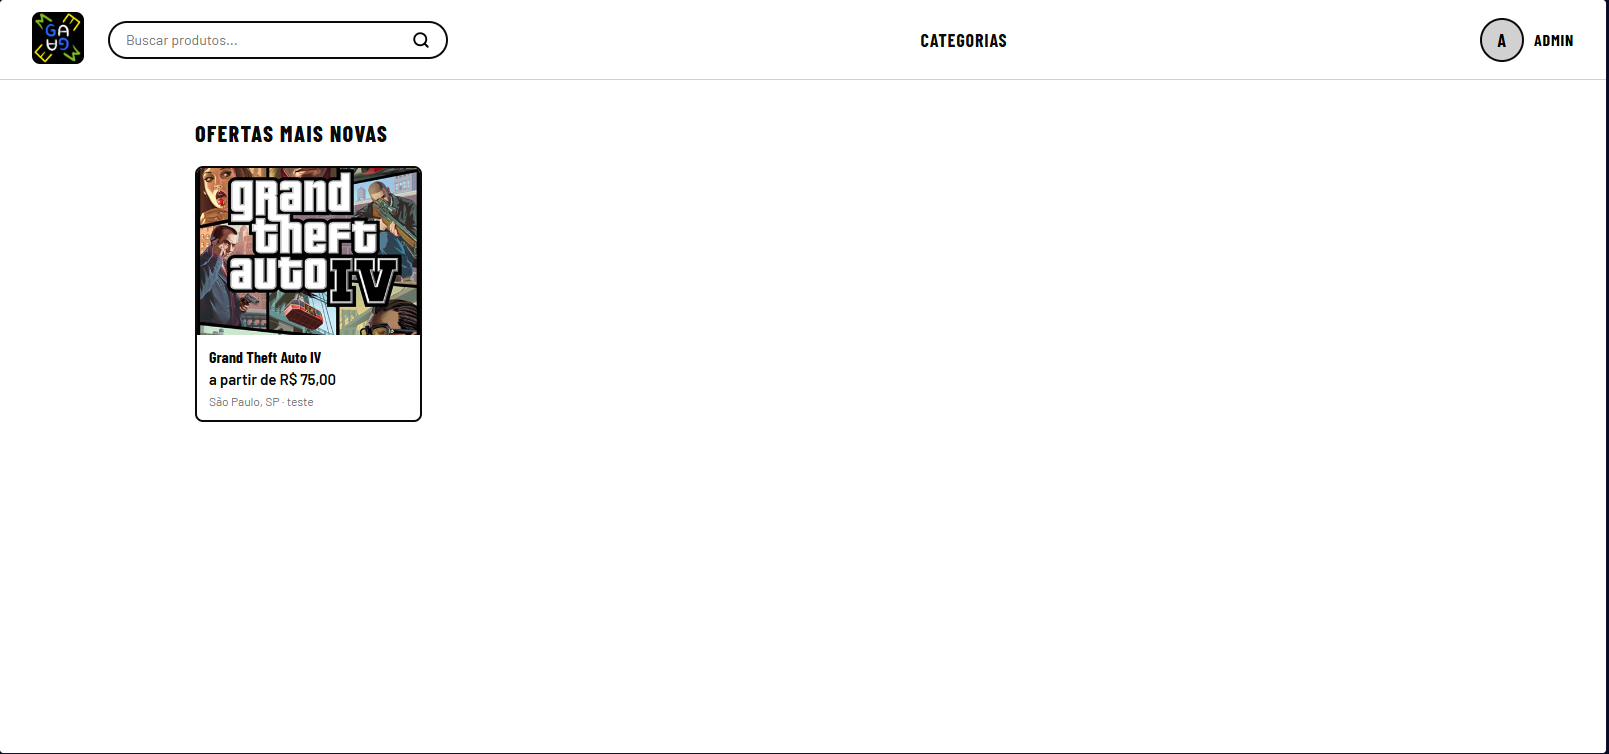
\includegraphics[width=0.95\textwidth]{images/image14.png}
  \caption{Captura de tela da \emph{home} do MegaGame}
  \label{fig:home}
  \legend{Fonte: Autor (2026).}
\end{figure}

\begin{figure}[htbp]
  \centering
  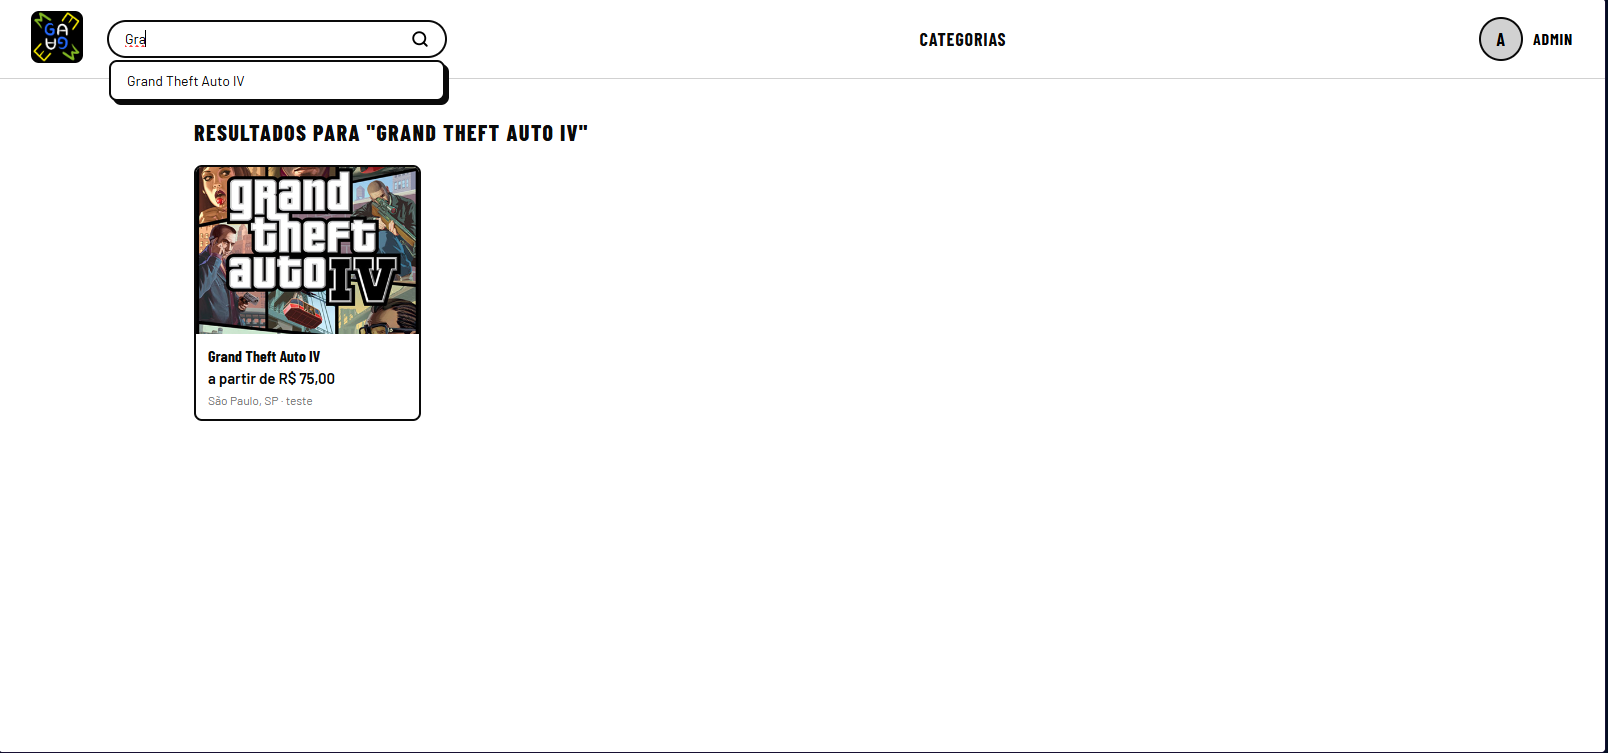
\includegraphics[width=0.95\textwidth]{images/image15.png}
  \caption{Captura de tela da pesquisa do MegaGame}
  \label{fig:pesquisa}
  \legend{Fonte: Autor (2026).}
\end{figure}

\begin{figure}[htbp]
  \centering
  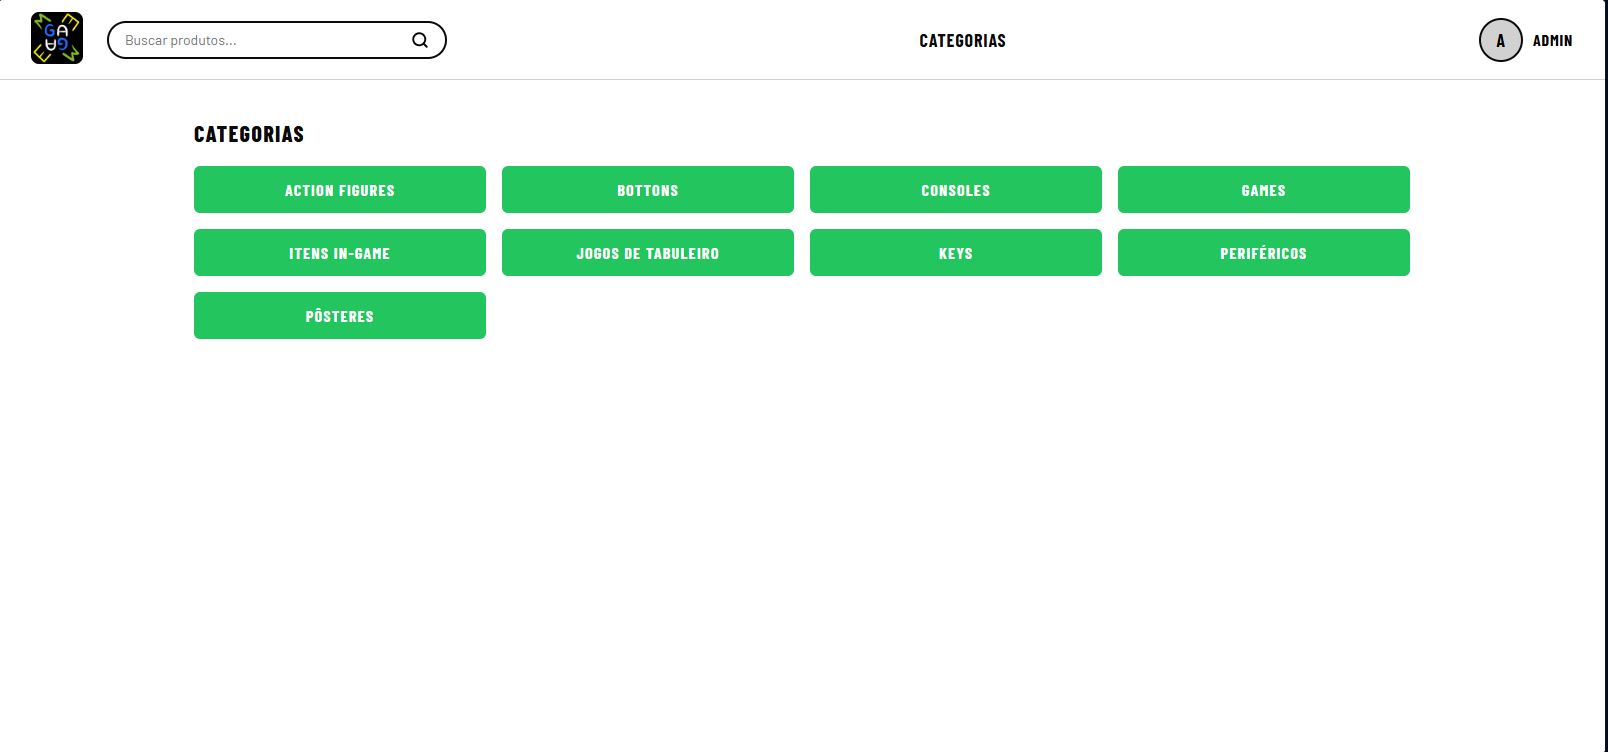
\includegraphics[width=0.95\textwidth]{images/image16.png}
  \caption{Captura de tela das categorias do MegaGame}
  \label{fig:categorias}
  \legend{Fonte: Autor (2026).}
\end{figure}

\begin{figure}[htbp]
  \centering
  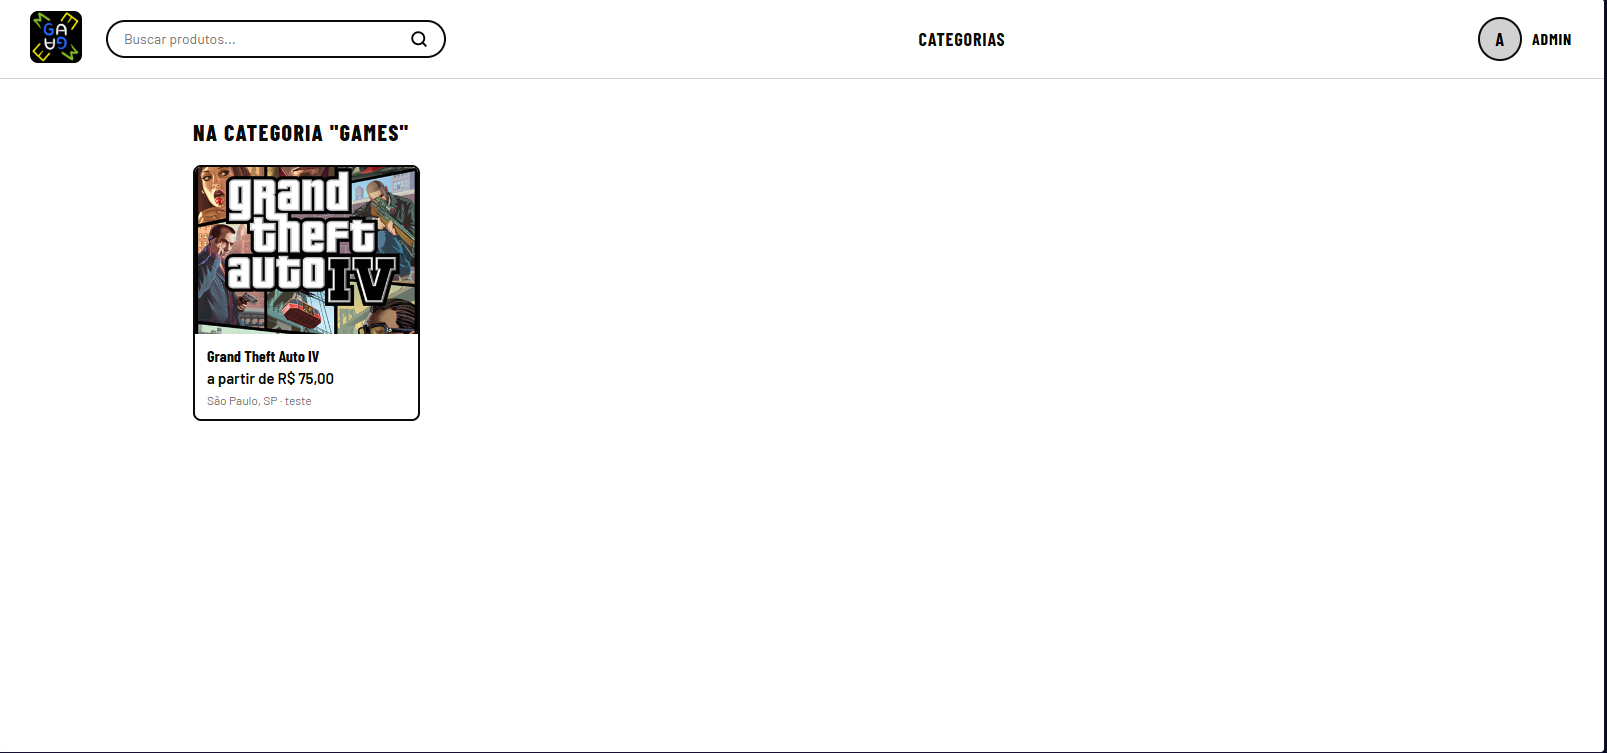
\includegraphics[width=0.95\textwidth]{images/image17.png}
  \caption{Captura de tela da busca por categoria do MegaGame}
  \label{fig:busca-por-categoria}
  \legend{Fonte: Autor (2026).}
\end{figure}

\begin{figure}[htbp]
  \centering
  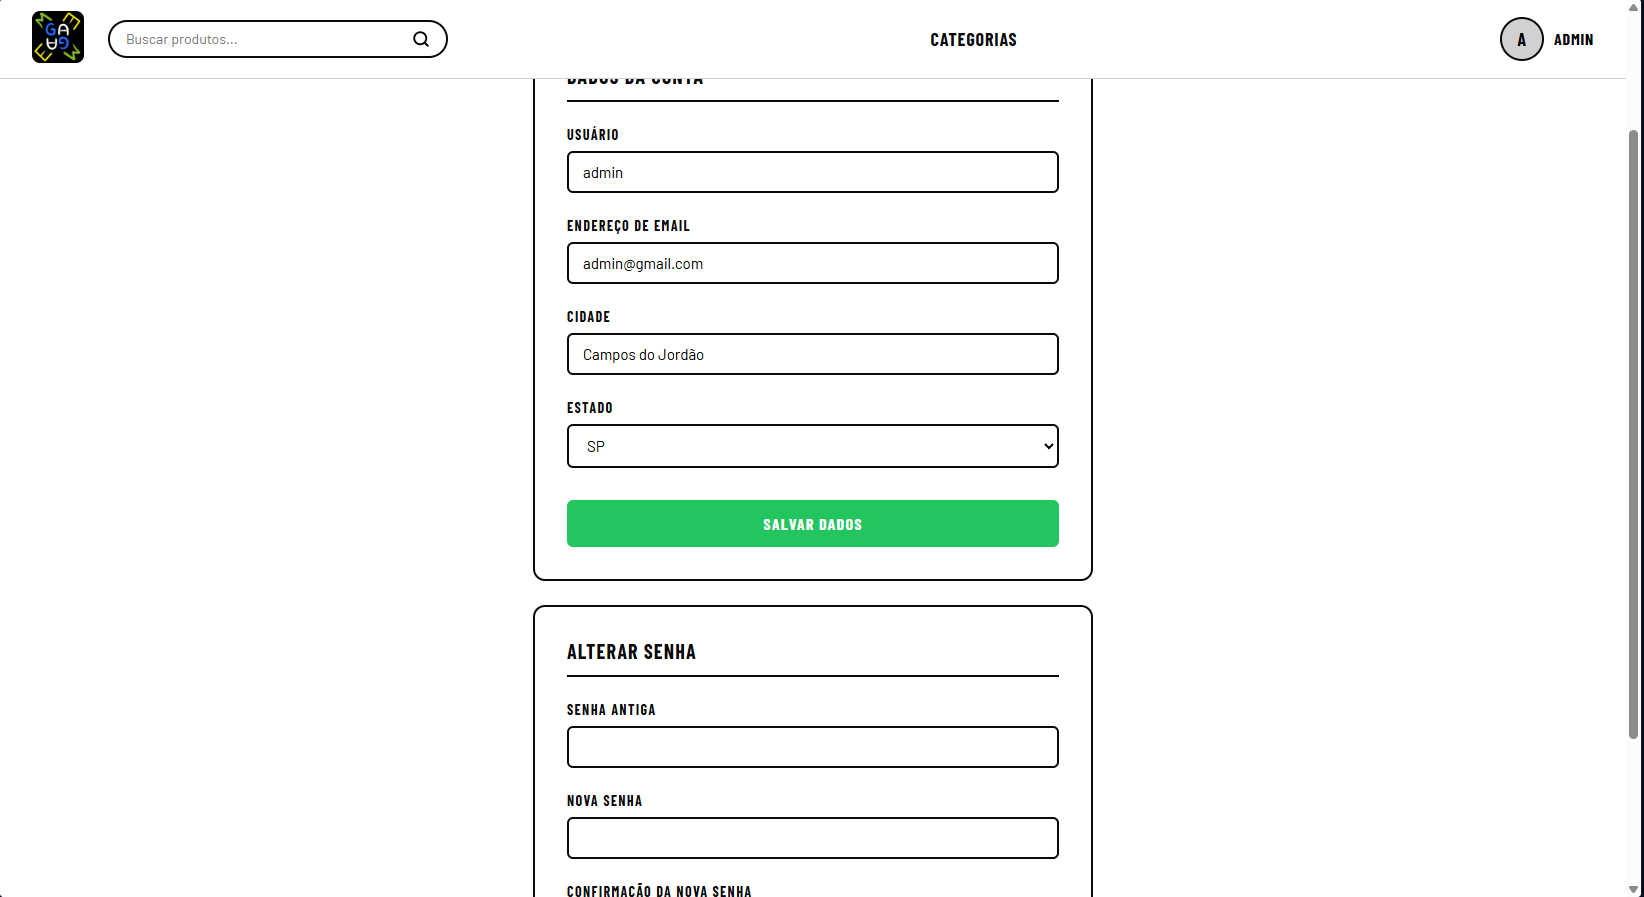
\includegraphics[width=0.95\textwidth]{images/image18.png}
  \caption{Captura de tela da edição de perfil do MegaGame}
  \label{fig:edicao-perfil}
  \legend{Fonte: Autor (2026).}
\end{figure}

\begin{figure}[htbp]
  \centering
  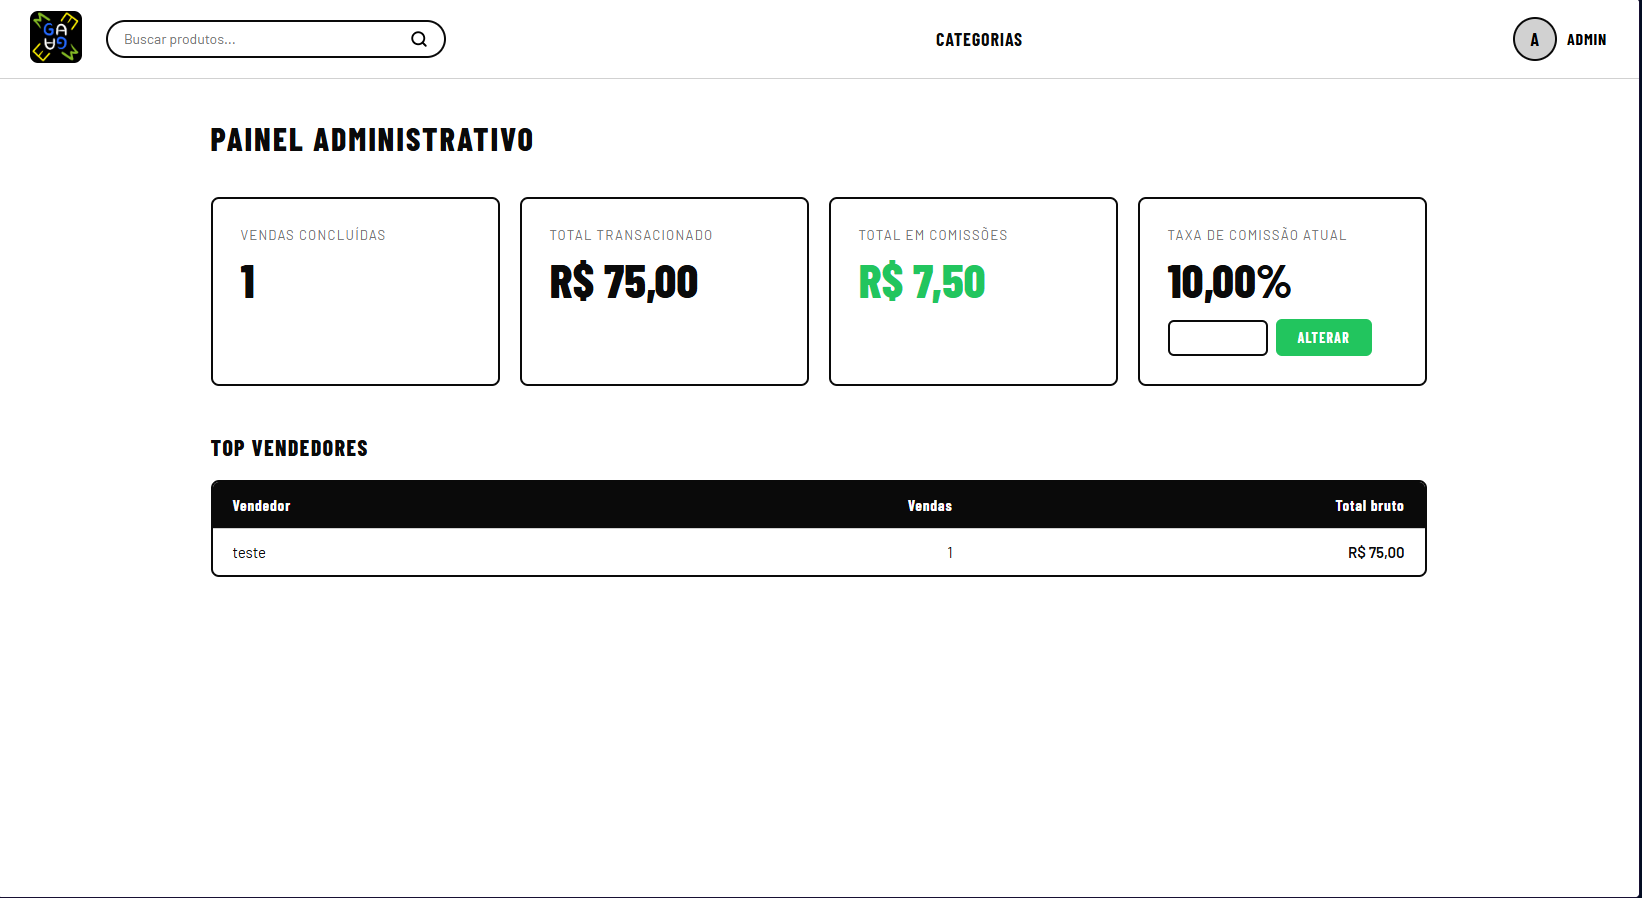
\includegraphics[width=0.95\textwidth]{images/image19.png}
  \caption{\emph{Dashboard} de gestor do MegaGame}
  \label{fig:dashboard-gestor}
  \legend{Fonte: Autor (2026).}
\end{figure}

\begin{figure}[htbp]
  \centering
  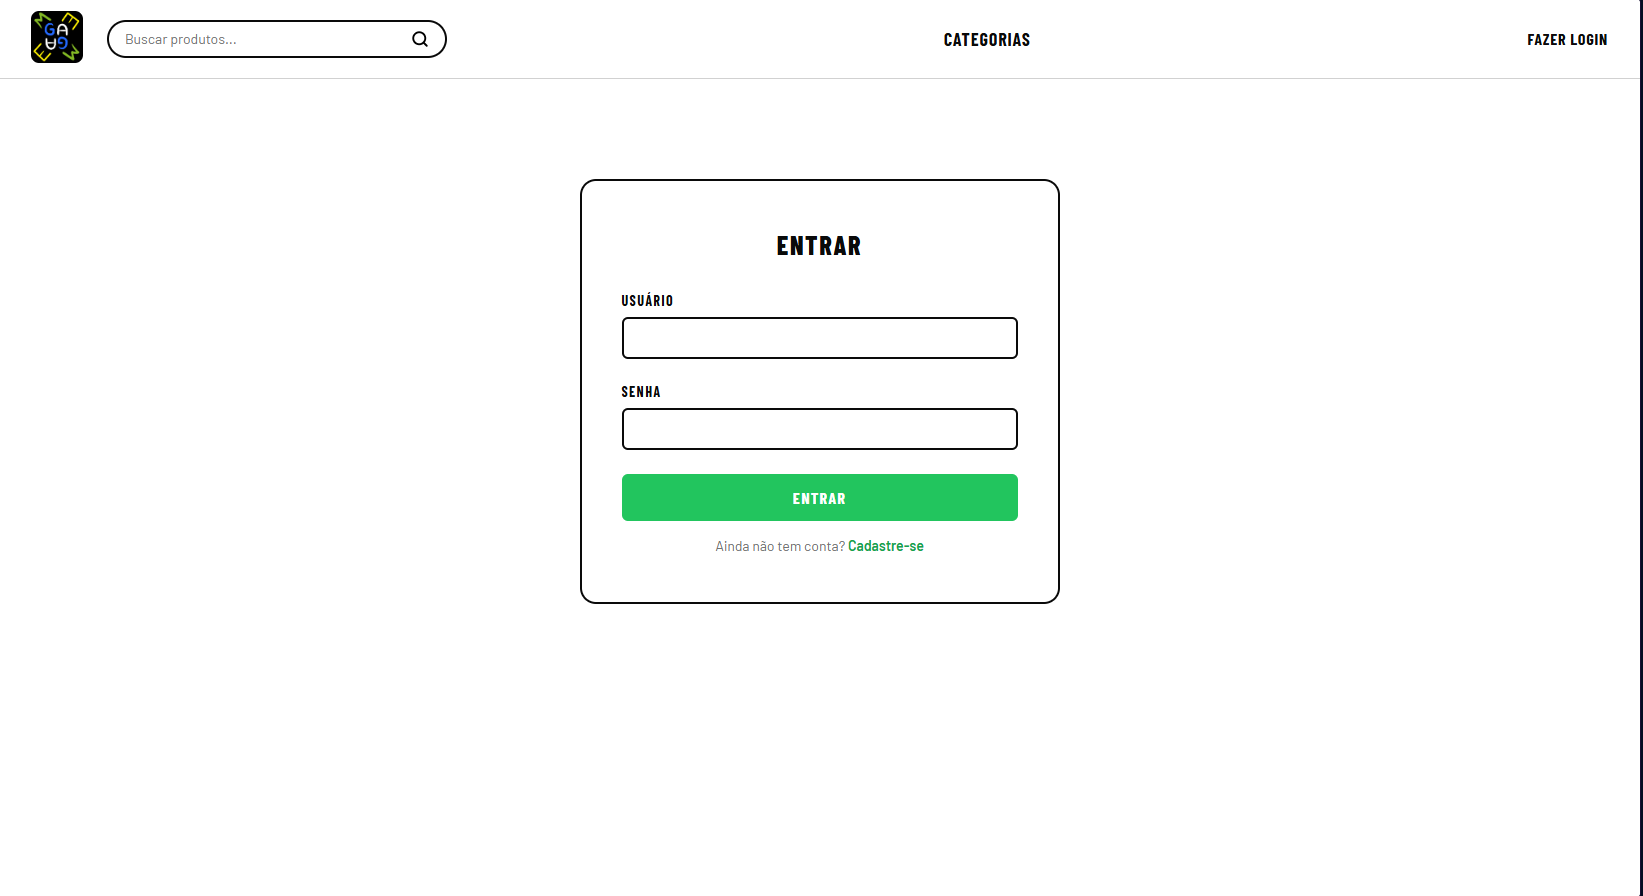
\includegraphics[width=0.95\textwidth]{images/image20.png}
  \caption{Captura de tela do \emph{login} do MegaGame}
  \label{fig:login}
  \legend{Fonte: Autor (2026).}
\end{figure}

\begin{figure}[htbp]
  \centering
  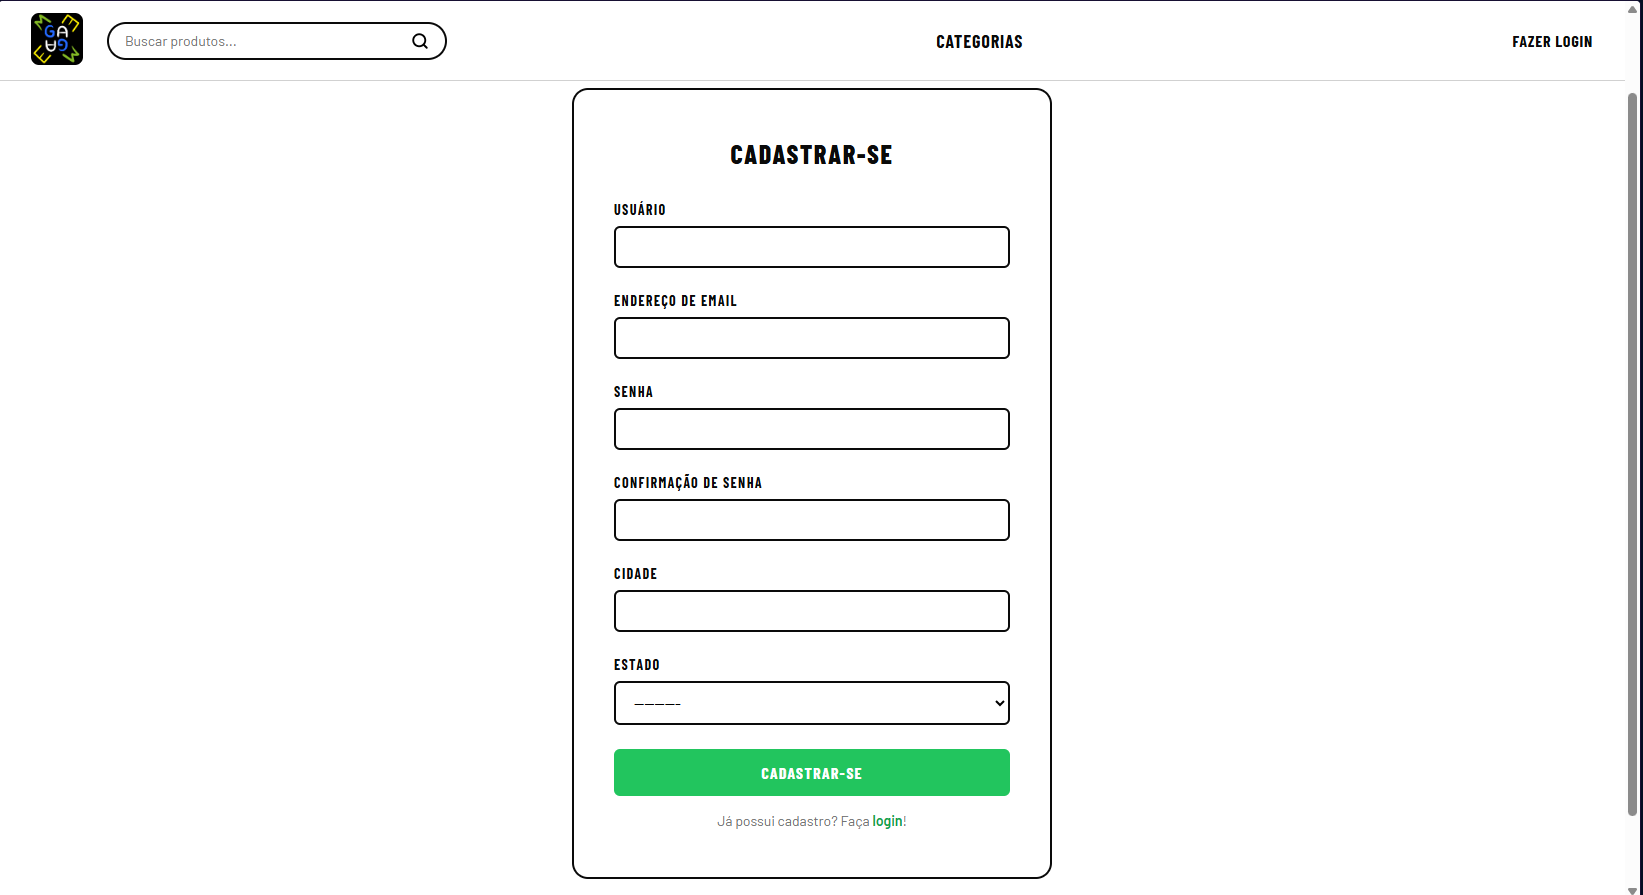
\includegraphics[width=0.95\textwidth]{images/image21.png}
  \caption{Captura de tela do cadastro do MegaGame}
  \label{fig:cadastro}
  \legend{Fonte: Autor (2026).}
\end{figure}

\begin{figure}[htbp]
  \centering
  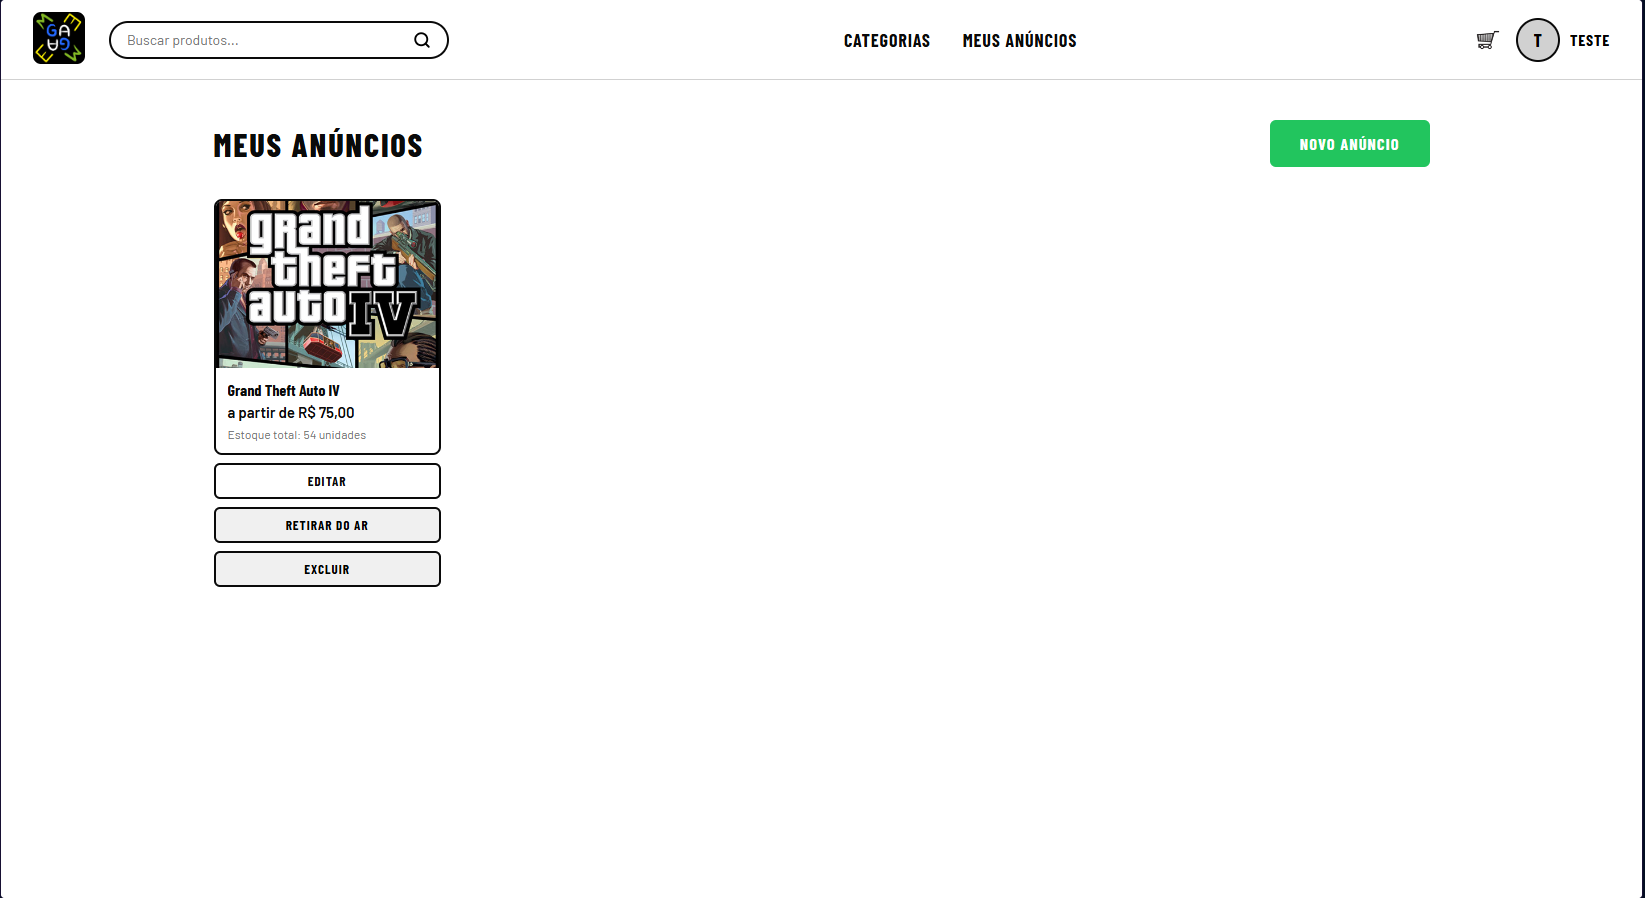
\includegraphics[width=0.95\textwidth]{images/image22.png}
  \caption{Captura de tela da lista de anúncios do MegaGame}
  \label{fig:lista-anuncios}
  \legend{Fonte: Autor (2026).}
\end{figure}

\begin{figure}[htbp]
  \centering
  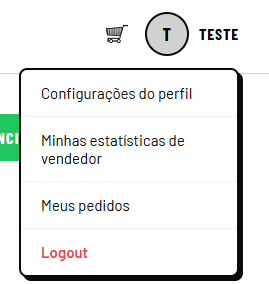
\includegraphics[width=0.55\textwidth]{images/image23.png}
  \caption{Captura de tela do \emph{dropdown menu} do MegaGame}
  \label{fig:dropdown-menu}
  \legend{Fonte: Autor (2026).}
\end{figure}

\begin{figure}[htbp]
  \centering
  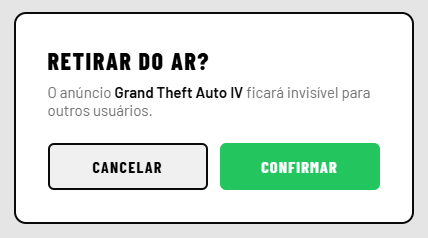
\includegraphics[width=0.75\textwidth]{images/image24.png}
  \caption{Captura de tela de um \emph{pop-up} de aviso do MegaGame}
  \label{fig:popup-aviso}
  \legend{Fonte: Autor (2026).}
\end{figure}

\begin{figure}[htbp]
  \centering
  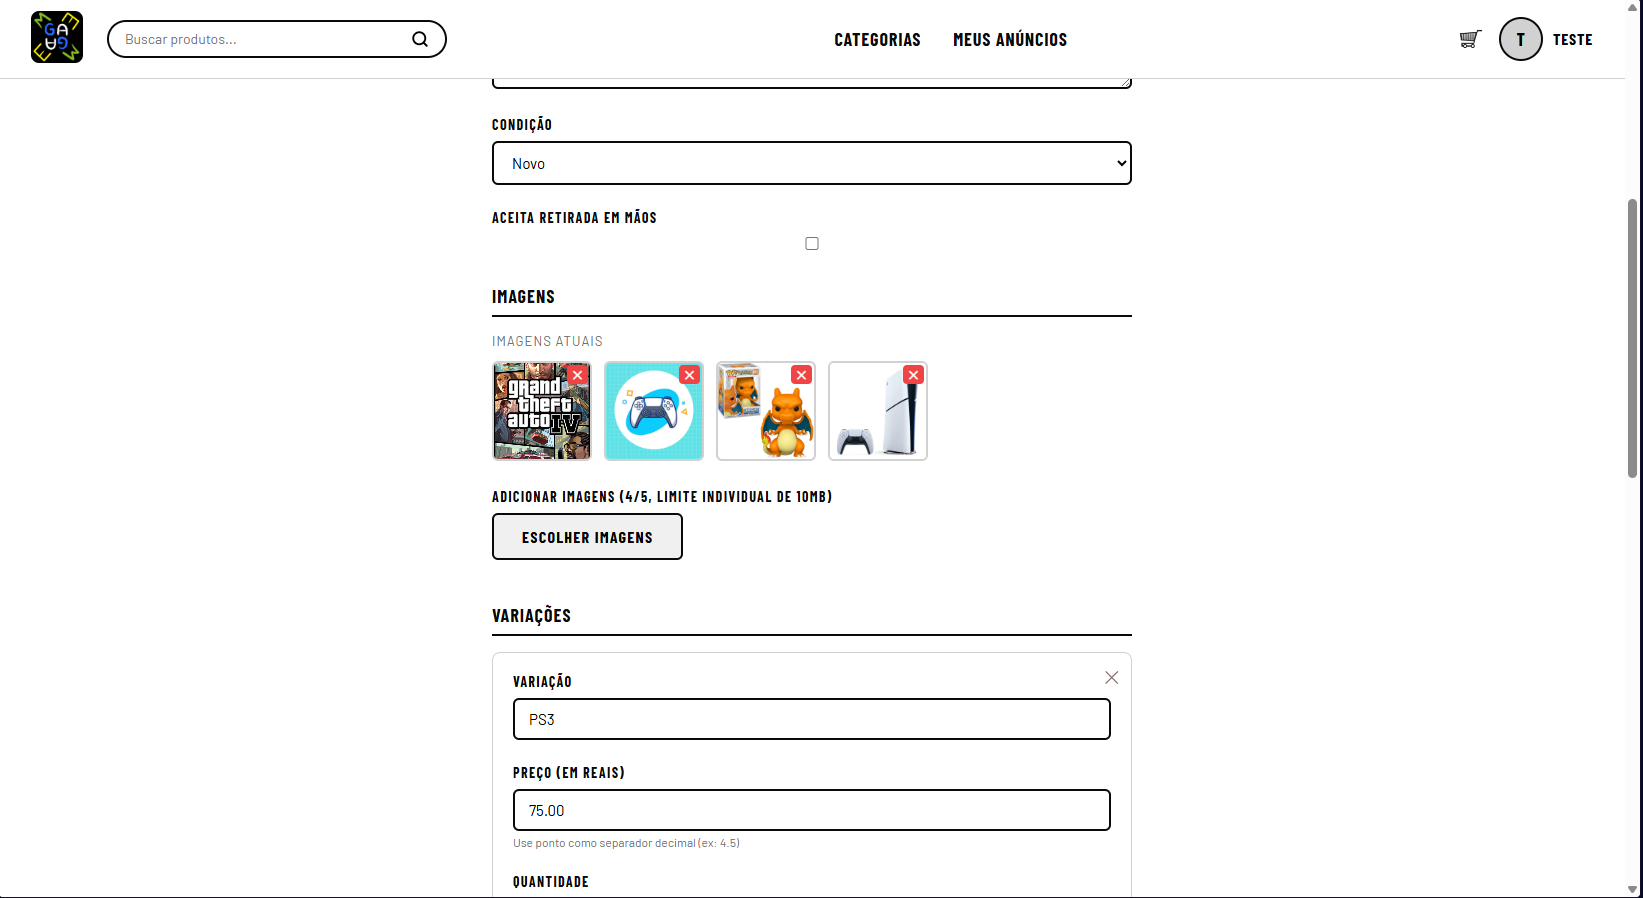
\includegraphics[width=0.95\textwidth]{images/image25.png}
  \caption{Captura de tela da edição de anúncio do MegaGame}
  \label{fig:edicao-anuncio}
  \legend{Fonte: Autor (2026).}
\end{figure}

\begin{figure}[htbp]
  \centering
  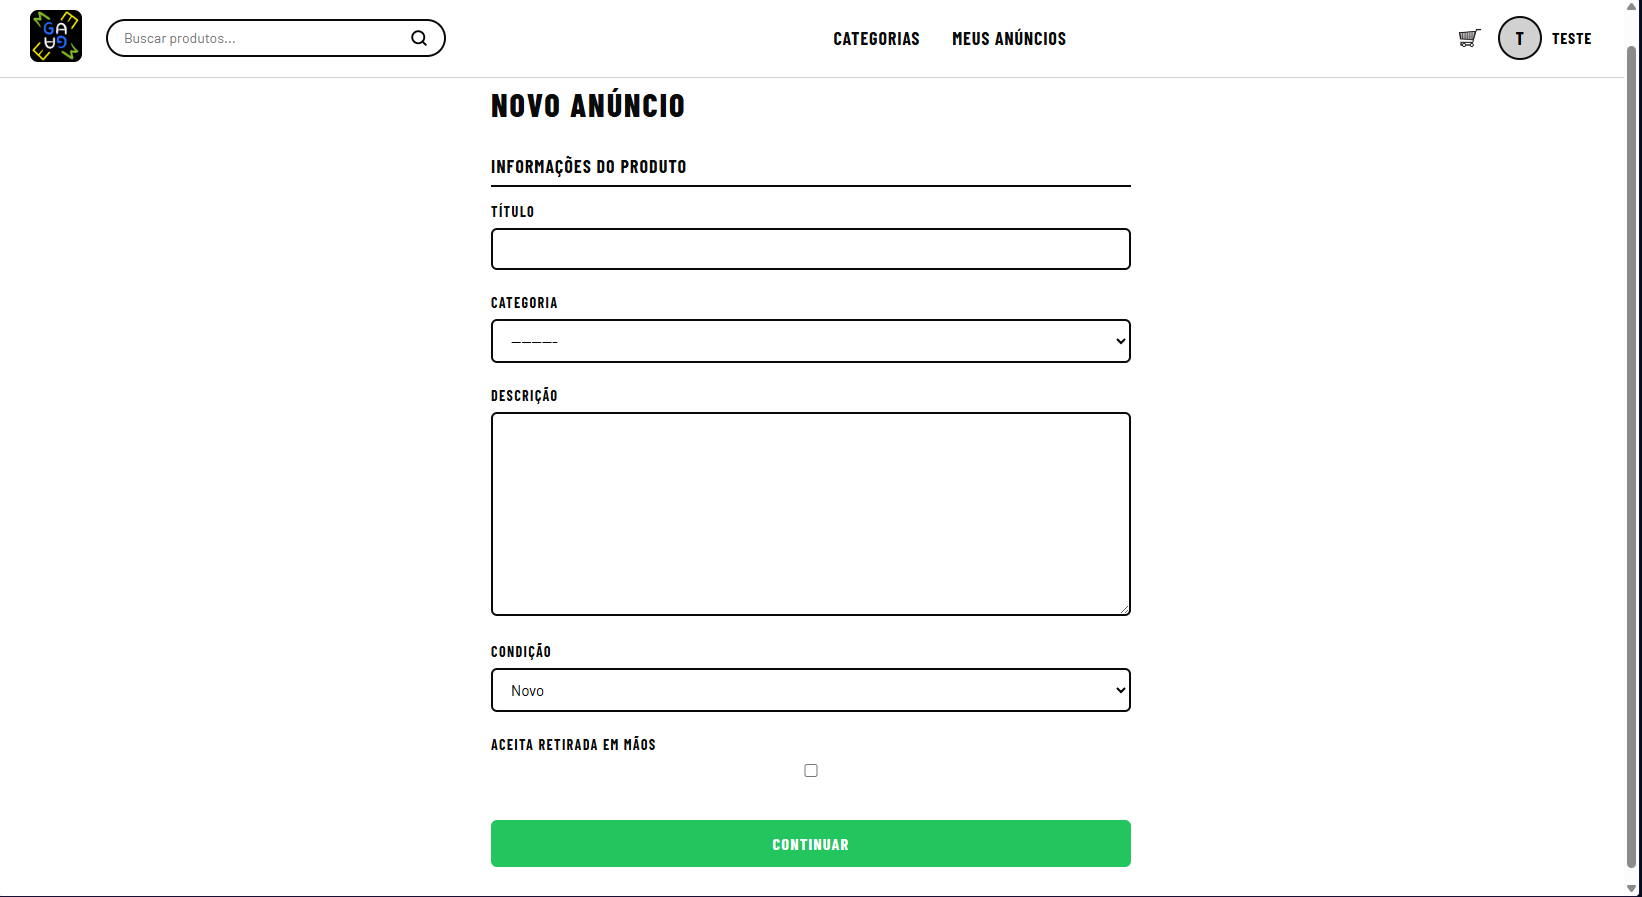
\includegraphics[width=0.95\textwidth]{images/image26.png}
  \caption{Captura de tela da criação de anúncio do MegaGame}
  \label{fig:criacao-anuncio}
  \legend{Fonte: Autor (2026).}
\end{figure}

\begin{figure}[htbp]
  \centering
  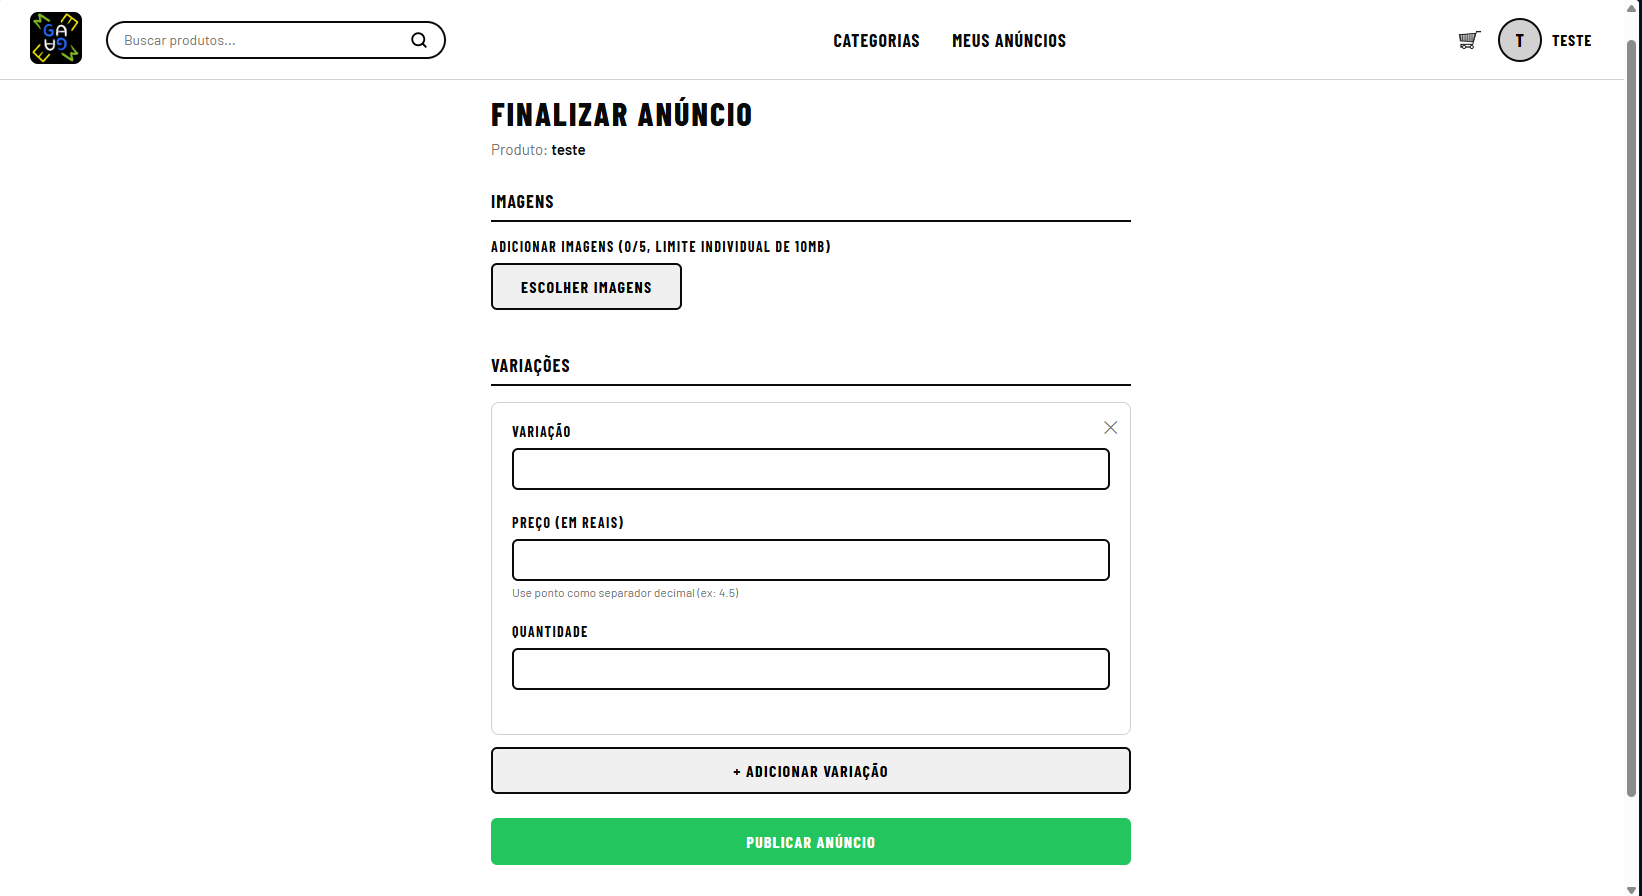
\includegraphics[width=0.95\textwidth]{images/image27.png}
  \caption{Criação de variações do MegaGame}
  \label{fig:criacao-variacoes}
  \legend{Fonte: Autor (2026).}
\end{figure}

\begin{figure}[htbp]
  \centering
  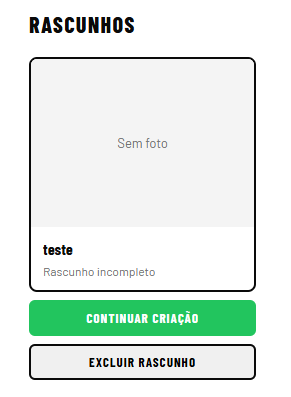
\includegraphics[width=0.6\textwidth]{images/image28.png}
  \caption{Rascunhos de anúncio do MegaGame}
  \label{fig:rascunhos-anuncio}
  \legend{Fonte: Autor (2026).}
\end{figure}

\begin{figure}[htbp]
  \centering
  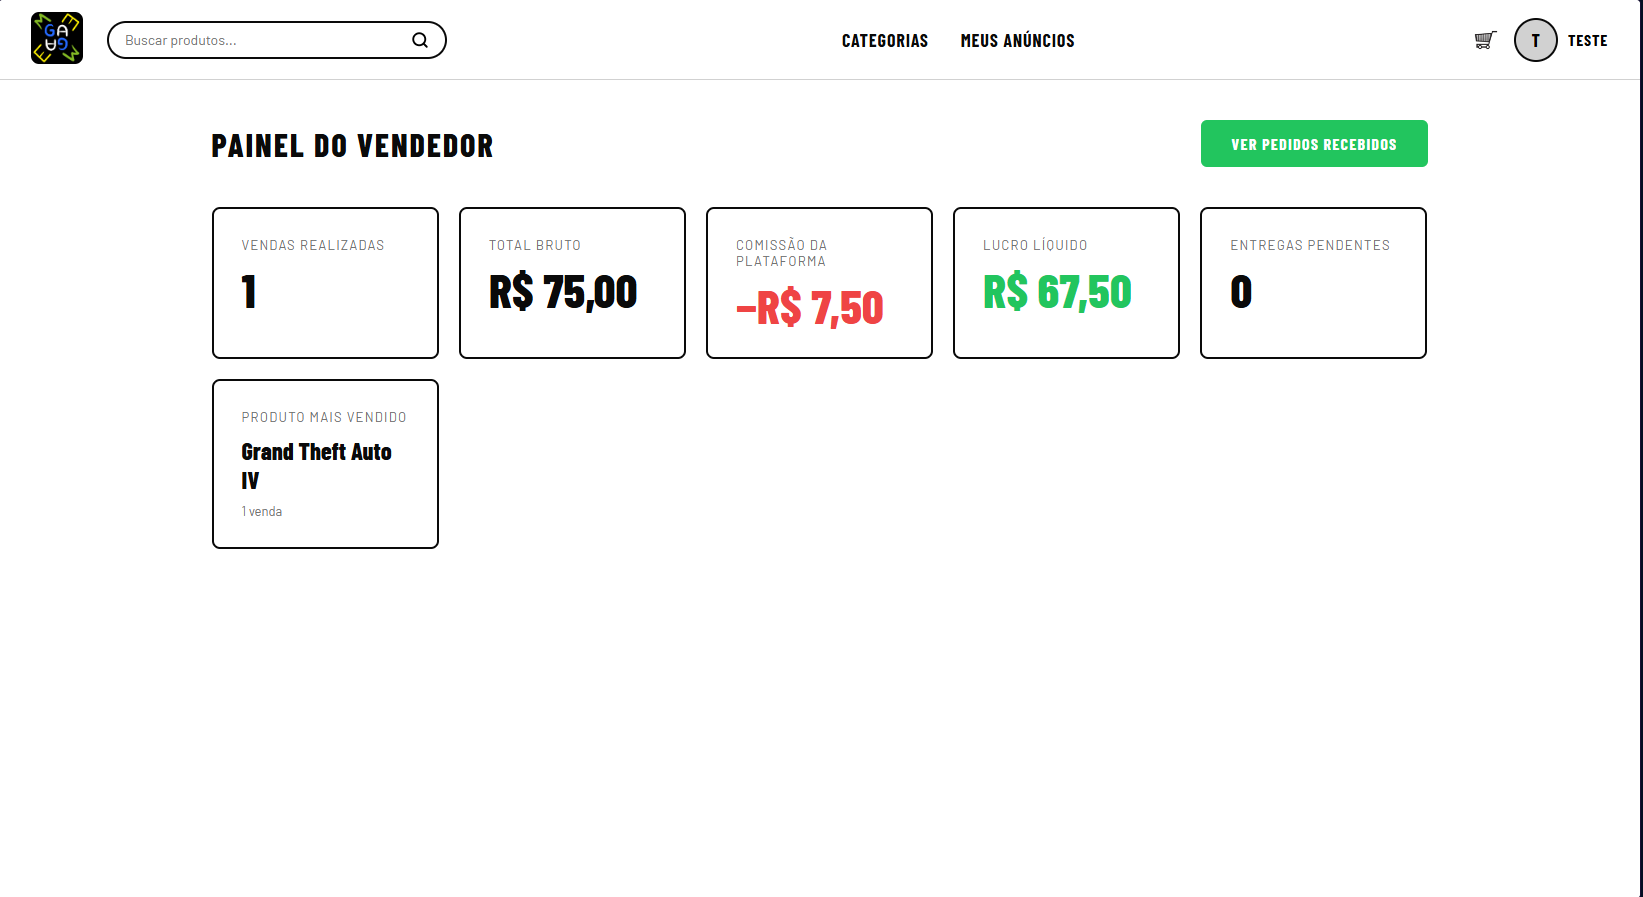
\includegraphics[width=0.95\textwidth]{images/image29.png}
  \caption{\emph{Dashboard} de vendedor do MegaGame}
  \label{fig:dashboard-vendedor}
  \legend{Fonte: Autor (2026).}
\end{figure}

\begin{figure}[htbp]
  \centering
  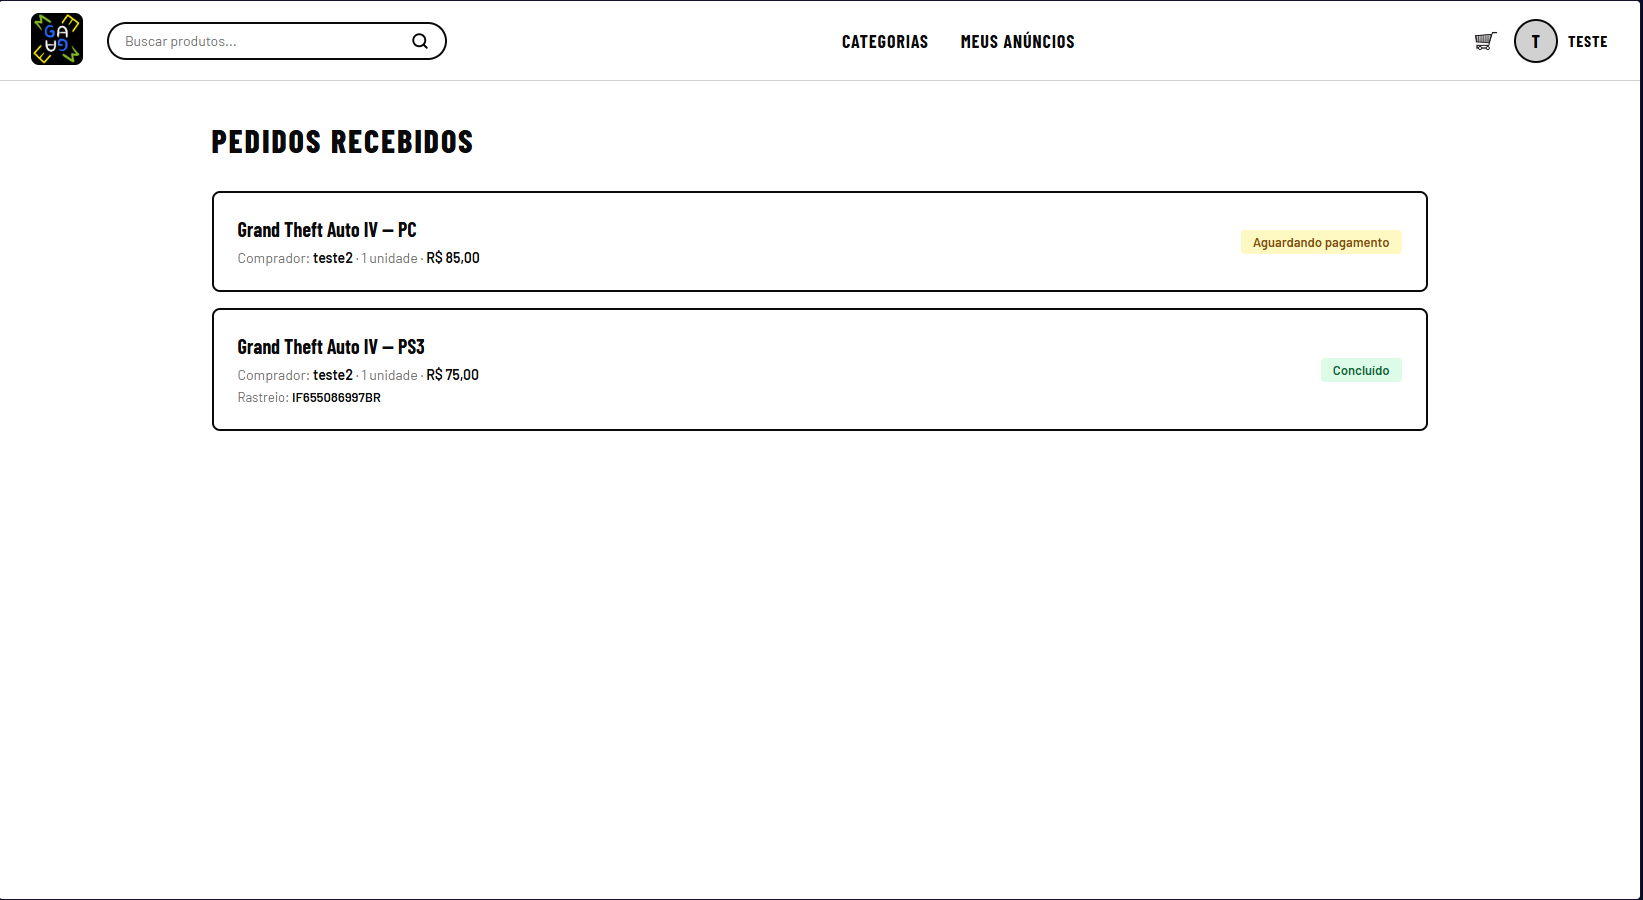
\includegraphics[width=0.95\textwidth]{images/image30.png}
  \caption{Captura de tela dos pedidos recebidos do MegaGame}
  \label{fig:pedidos-recebidos}
  \legend{Fonte: Autor (2026).}
\end{figure}

\begin{figure}[htbp]
  \centering
  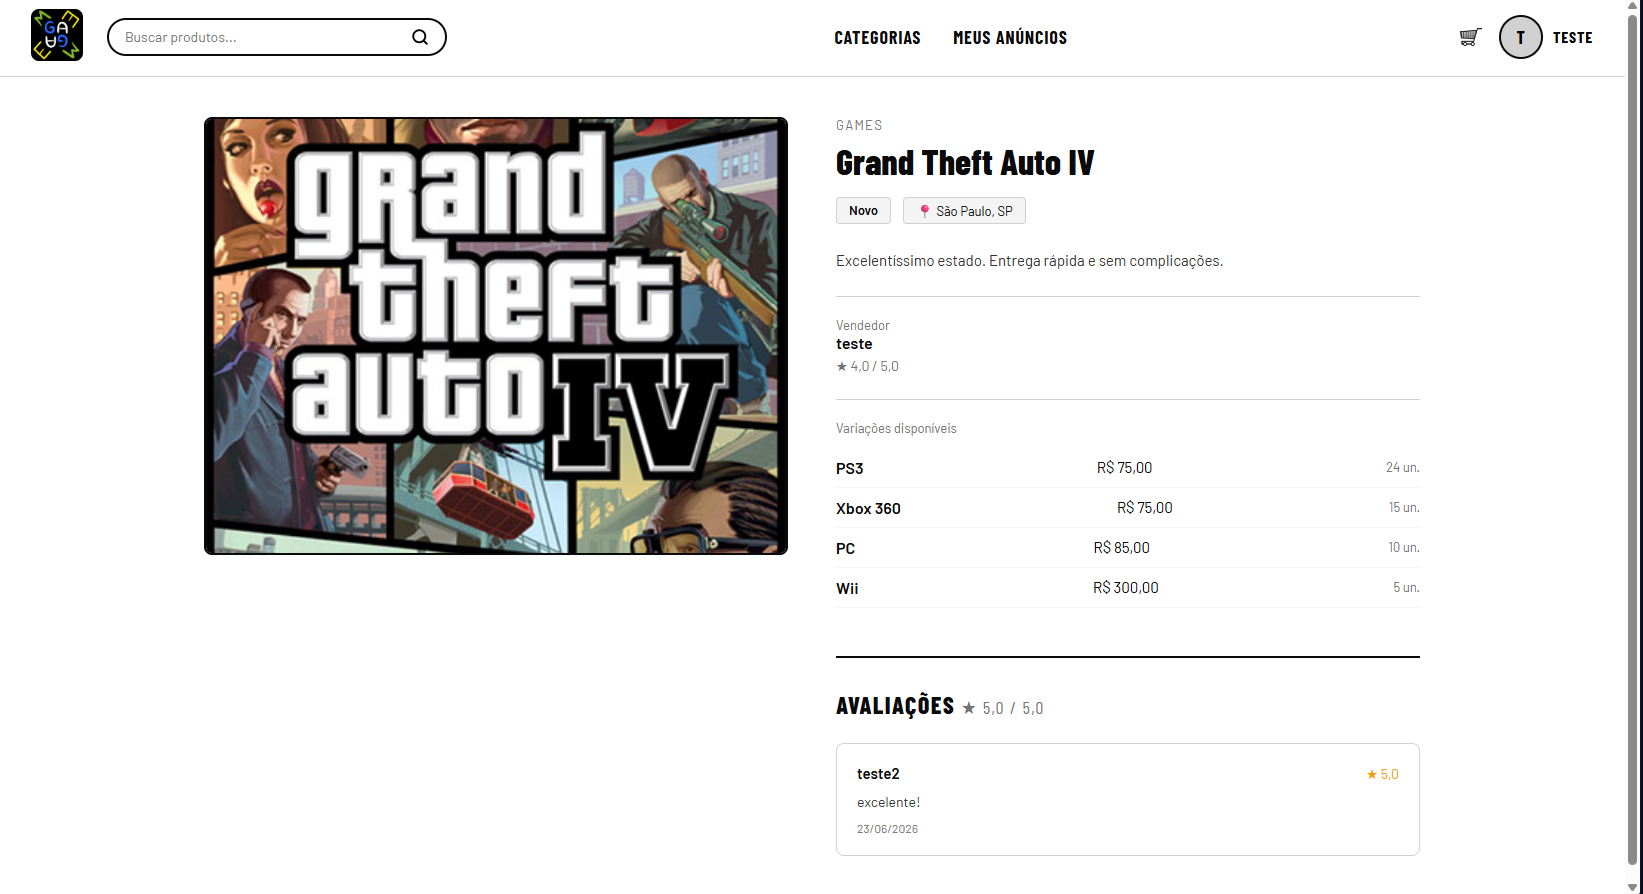
\includegraphics[width=0.95\textwidth]{images/image31.png}
  \caption{Captura de tela dos anúncios do MegaGame}
  \label{fig:anuncios}
  \legend{Fonte: Autor (2026).}
\end{figure}

\begin{figure}[htbp]
  \centering
  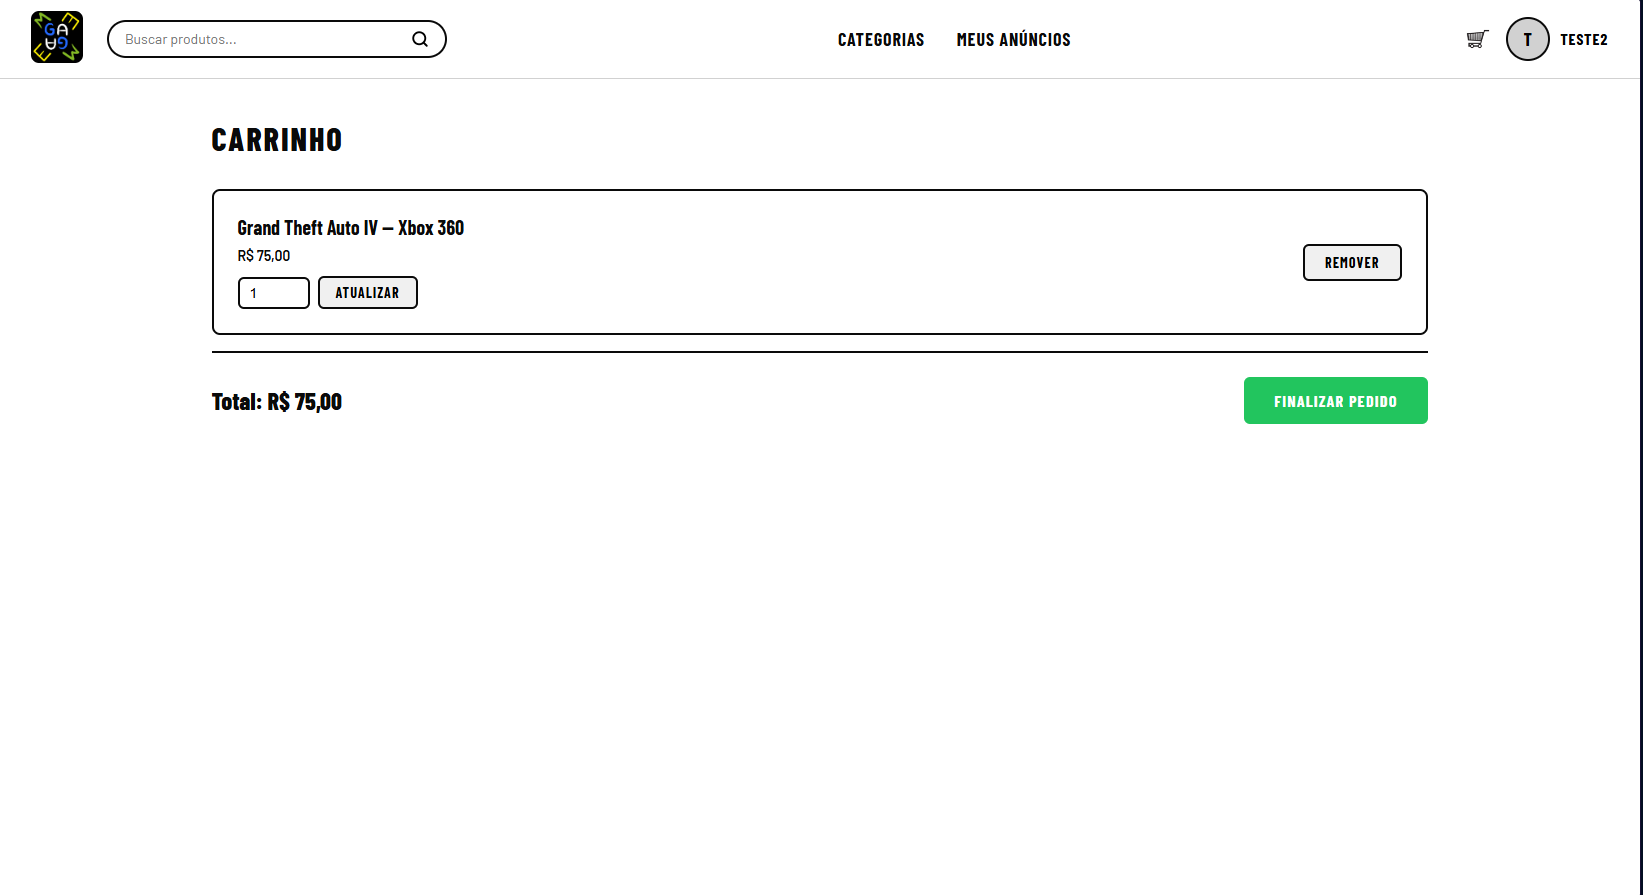
\includegraphics[width=0.95\textwidth]{images/image32.png}
  \caption{Captura de tela do carrinho do MegaGame}
  \label{fig:carrinho}
  \legend{Fonte: Autor (2026).}
\end{figure}

\begin{figure}[htbp]
  \centering
  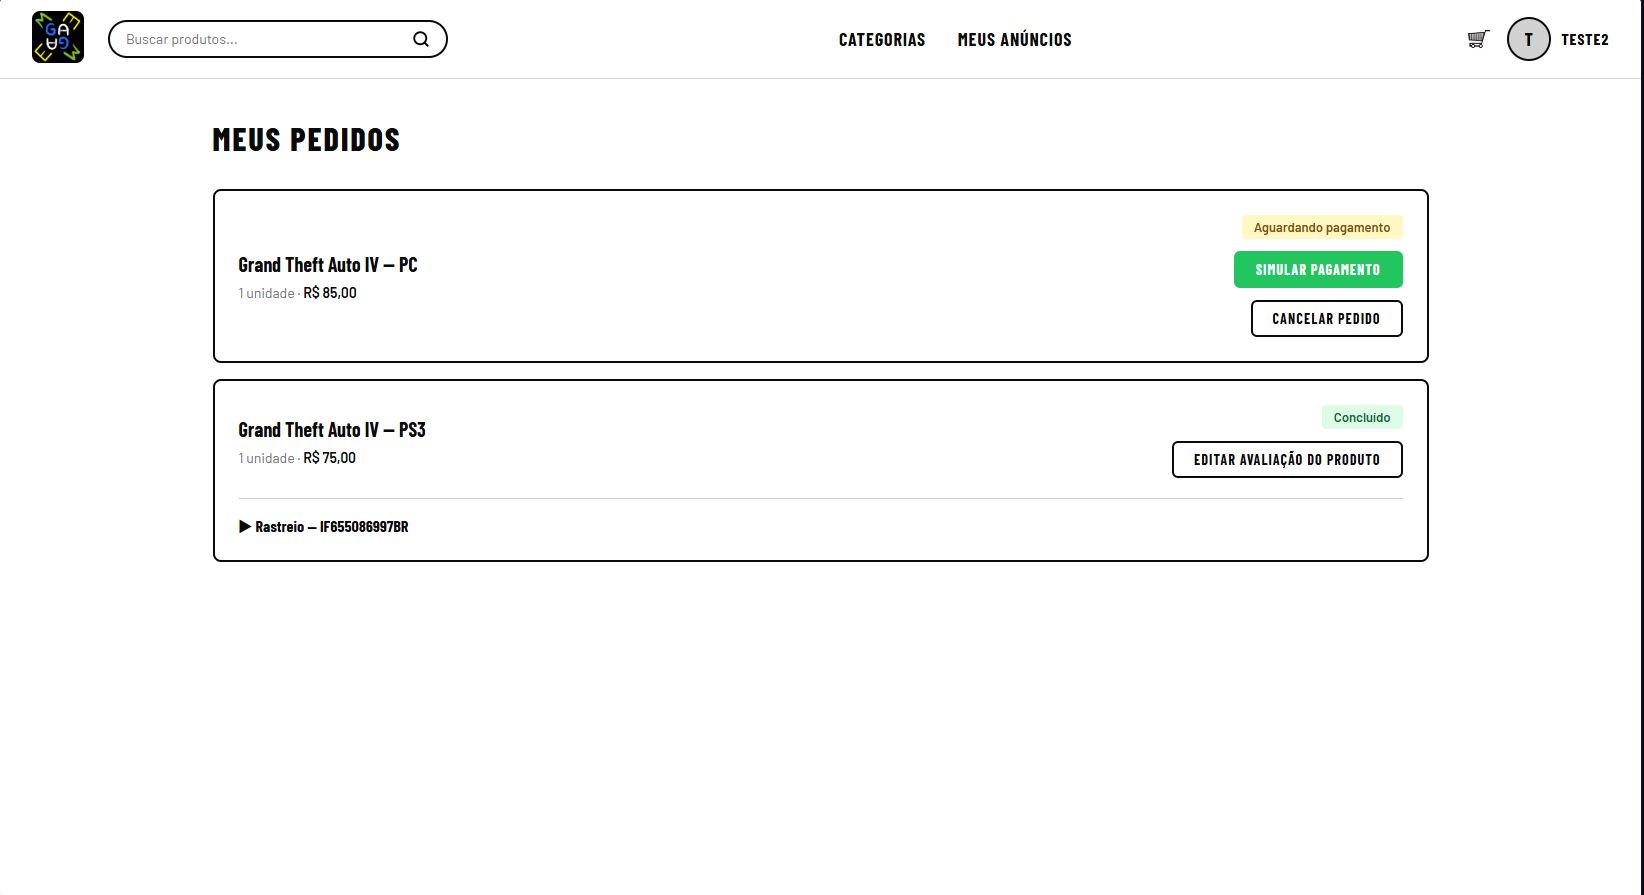
\includegraphics[width=0.95\textwidth]{images/image33.png}
  \caption{Captura de tela dos pedidos feitos do MegaGame}
  \label{fig:pedidos-feitos}
  \legend{Fonte: Autor (2026).}
\end{figure}

\begin{figure}[htbp]
  \centering
  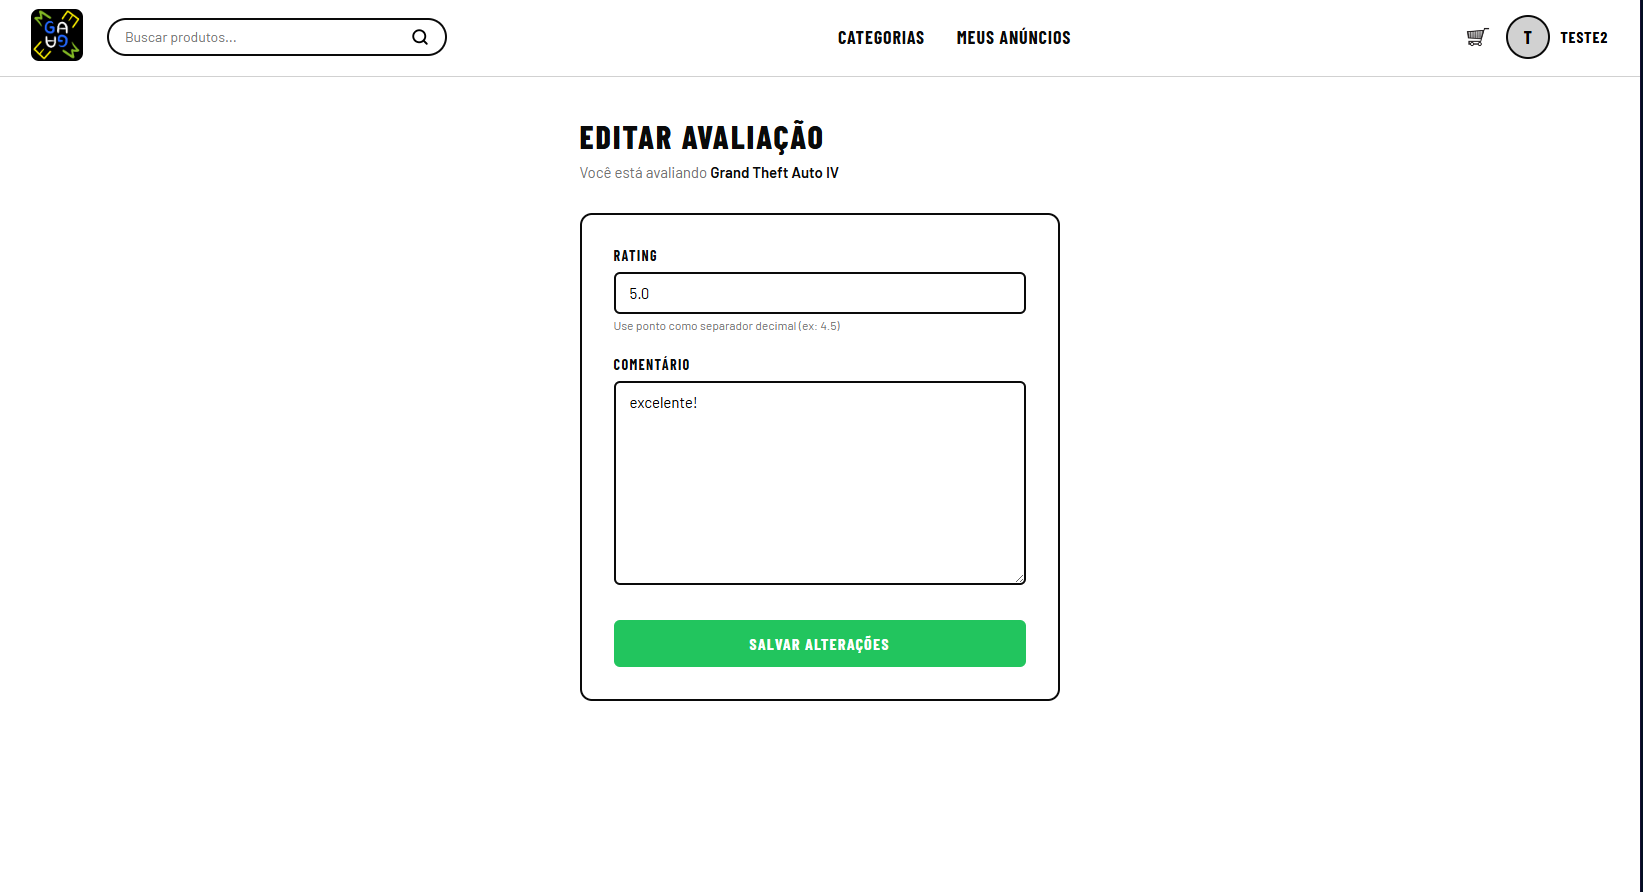
\includegraphics[width=0.95\textwidth]{images/image34.png}
  \caption{Avaliação de produto do MegaGame}
  \label{fig:avaliacao-produto}
  \legend{Fonte: Autor (2026).}
\end{figure}

\begin{figure}[htbp]
  \centering
  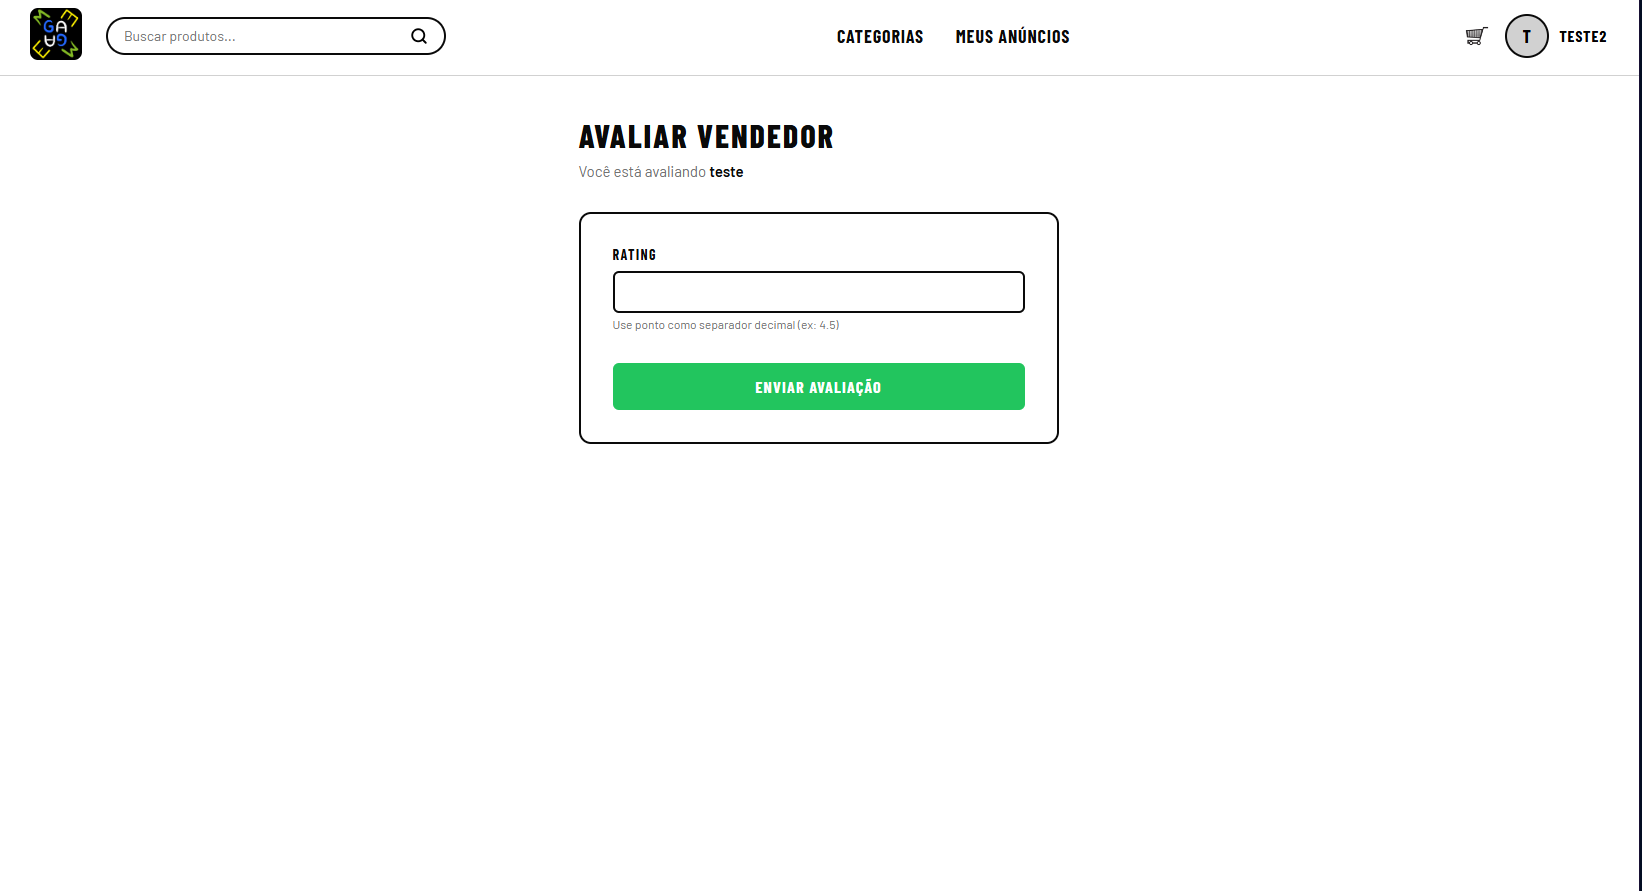
\includegraphics[width=0.95\textwidth]{images/image35.png}
  \caption{Avaliação de vendedor do MegaGame}
  \label{fig:avaliacao-vendedor}
  \legend{Fonte: Autor (2026).}
\end{figure}

\section{Implementação}

O projeto foi construído no Visual Studio Code, IDE da Microsoft. Para
rodar o site a partir dele, é necessário primeiramente instalar as
dependências do projeto (a partir do arquivo requirements.txt) em um
ambiente virtual (venv), configurar core/settings.py e colocar as
informações necessárias em um arquivo .env (os possíveis campos estão
especificados em .env.example) para que o sistema ``aponte'' pro banco
de dados, executar o comando ``python manage.py migrate'' no terminal do
VS Code para que o banco sendo utilizado receba todas as tabelas
necessárias e então executar o comando ``python manage.py runserver''
quando for necessário inicializar o servidor local.

manage.py é um arquivo na raiz do repositório que, conforme seu nome
indica, é responsável por administrar toda a questão da renderização do
código (lembrando da prática do SSR empregada aqui) quando ``invocado''.
Apesar de funcionar apenas de forma local no momento, a infraestrutura
já foi projetada para estar pronta pra um \emph{deploy} real na
\emph{web} conforme o projeto avança.

\chapter{Conclusão}

Retomando as premissas deste trabalho, o objetivo era apresentar o
desenvolvimento do MegaGame, um \emph{marketplace} C2C projetado
especificamente para preencher uma lacuna identificada no cenário
nacional de jogos eletrônicos, que era a falta de uma plataforma de
comércio dedicada a esse segmento. Através dos passos detalhados no
decorrer do documento, foi possível projetar e implementar um espaço
otimizado para o comércio de produtos relacionados a jogos, sendo este
funcional, seguro e escalável.

As escolhas metodológicas tomadas para cumprir a meta obtiveram êxito.
No \emph{back end}, o Django com SSR garantiu robustez e estabilidade,
enquanto o Supabase proporcionou uma infraestrutura de dados confiável e
pronta pra \emph{deploy}. Assim, atenderam-se tanto as necessidades
operacionais comuns quanto os princípios guiadores da engenharia de
\emph{software}.

Adicionalmente, a arquitetura escolhida, tal como o uso do UML para
mapear as funcionalidades do sistema, garante que seja possível evoluir
a ideia cada vez mais confome o tempo, independente de quem esteja no
comando, ao fornecer \emph{insights} claros e objetivos sobre como tudo
é operado.

Em suma, o projeto demonstra a viabilidade técnica de uma solução
comercial voltada ao público \emph{gamer}, integrando conceitos teóricos
de gestão de projetos com ferramentas consolidadas do mercado
tecnológico. Com isso, o MegaGame se estabelece como uma resposta
prática a uma oportunidade de mercado atual e também como uma aplicação
pronta para ser adaptada de acordo com futuras demandas do setor.

\postextual

\bibliography{referencias}

\end{document}
